%%%%%%%%%%%%%%%%%%%%%%%%%%%%%%%%%%%%%%%%%%%%%%%%%%%%%%%%%%%%%%%%%%%%%%
% Overleaf (WriteLaTeX) Example: Molecular Chemistry Presentation
%
% Source: http://www.overleaf.com
%
% In these slides we show how Overleaf can be used with standard 
% chemistry packages to easily create professional presentations.
% 
% Feel free to distribute this example, but please keep the referral
% to overleaf.com
% 
%%%%%%%%%%%%%%%%%%%%%%%%%%%%%%%%%%%%%%%%%%%%%%%%%%%%%%%%%%%%%%%%%%%%%%
% How to use Overleaf: 
%
% You edit the source code here on the left, and the preview on the
% right shows you the result within a few seconds.
%
% Bookmark this page and share the URL with your co-authors. They can
% edit at the same time!
%
% You can upload figures, bibliographies, custom classes and
% styles using the files menu.
%
% If you're new to LaTeX, the wikibook is a great place to start:
% http://en.wikibooks.org/wiki/LaTeX
%
%%%%%%%%%%%%%%%%%%%%%%%%%%%%%%%%%%%%%%%%%%%%%%%%%%%%%%%%%%%%%%%%%%%%%%

\documentclass{beamer}

% For more themes, color themes and font themes, see:
% http://deic.uab.es/~iblanes/beamer_gallery/index_by_theme.html
%
\mode<presentation>
{
  \usetheme{Madrid}       % or try default, Darmstadt, Warsaw, ...
  \usecolortheme{default} % or try albatross, beaver, crane, ...
  \usefonttheme{serif}    % or try default, structurebold, ...
  \setbeamertemplate{navigation symbols}{}
  \setbeamertemplate{caption}[numbered]
} 

\usepackage[english]{babel}
\usepackage[utf8x]{inputenc}
\usepackage{chemfig}
\usepackage[version=3]{mhchem}

% On Overleaf, these lines give you sharper preview images.
% You might want to `comment them out before you export, though.
\usepackage{pgfpages}
\pgfpagesuselayout{resize to}[%
  physical paper width=8in, physical paper height=6in]

%==================================
\usepackage{subfigure}
\usepackage[]{algorithm2e}
\usepackage{apalike}
%\usepackage{SCITEPRESS}
%\usepackage{algorithm}
%\usepackage{algorithmic}

% \REDCOMMENT{text}
\newcommand{\REDCOMMENT}[1]{\color{red}{#1}\color{black}}

% \BLUECOMMENT{text}
\newcommand{\BLUECOMMENT}[1]{\color{blue}{#1}\color{black}}

%==================================

% Here's where the presentation starts, with the info for the title slide
\title[My Computer Graphics Background]{A presentation on my background in computer graphics}
\author{M. Mostajab}
\institute{\url{www.mmostajab.com}}
\date{\today}

\begin{document}

\begin{frame}
  \titlepage
\end{frame}

% These three lines create an automatically generated table of contents.
\begin{frame}{Outline}
  \tableofcontents
\end{frame}

\section{Introduction}

\begin{frame}{About Me...}
	\begin{tikzpicture}[overlay, remember picture]
		\node[anchor=north east, xshift=-30pt,yshift=-55pt]
		at(current page.north east){
			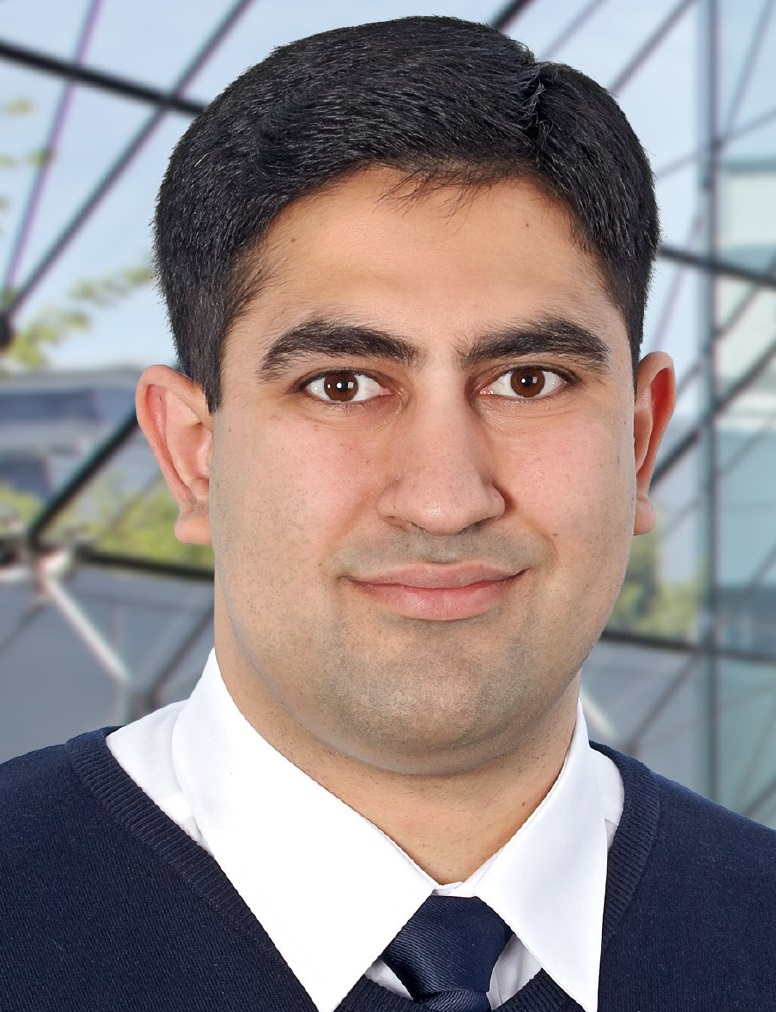
\includegraphics[width=30mm]{figures/photo.jpg}
		};
	\end{tikzpicture}

	\begin{itemize}
		\item My name is \textbf{Morteza Mostajab}
		\item B.Sc. Computer Engineering at\\ \textit{Hamedan University of Technology, Iran}
		\item M.Sc. Computer Science at\\ \textit{Technische Universit{\"a}t M{\"unchen}}
		\item Working as Researcher at\\ \textit{Fraunhofer IGD, Darmstadt}
		\item Research interests:\\
		    \textit{Real-time physically-based rendering} \\
			\textit{(Rasterization-based or Ray-tracing)}\\
			\textit{Virtual reality}\\
			\textit{Computer graphics and visualization}\\
			\textit{Game Programming}
		   
	\end{itemize}
\end{frame}

\begin{frame}{Inspiration}
	
	\begin{itemize}
		\item Games, Animations, Movies with Special Effects,...
			\begin{figure}
			\centering
			\subfigure[Last Ninja 3]{
				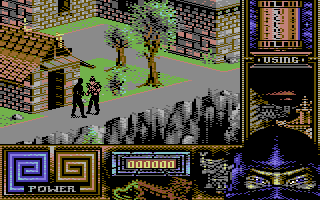
\includegraphics[width=0.19\linewidth]{figures/LastNinja.png}
			}
			%\subfigure[Warcraft 2]{
			%	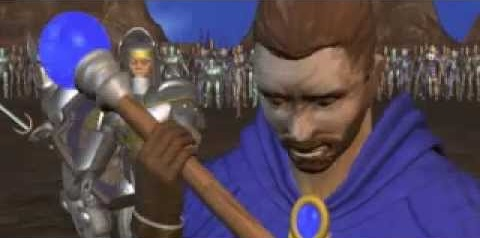
\includegraphics[width=0.2\linewidth]{figures/warcraft2.jpg}
			%}
			\subfigure[Gears of War]{
				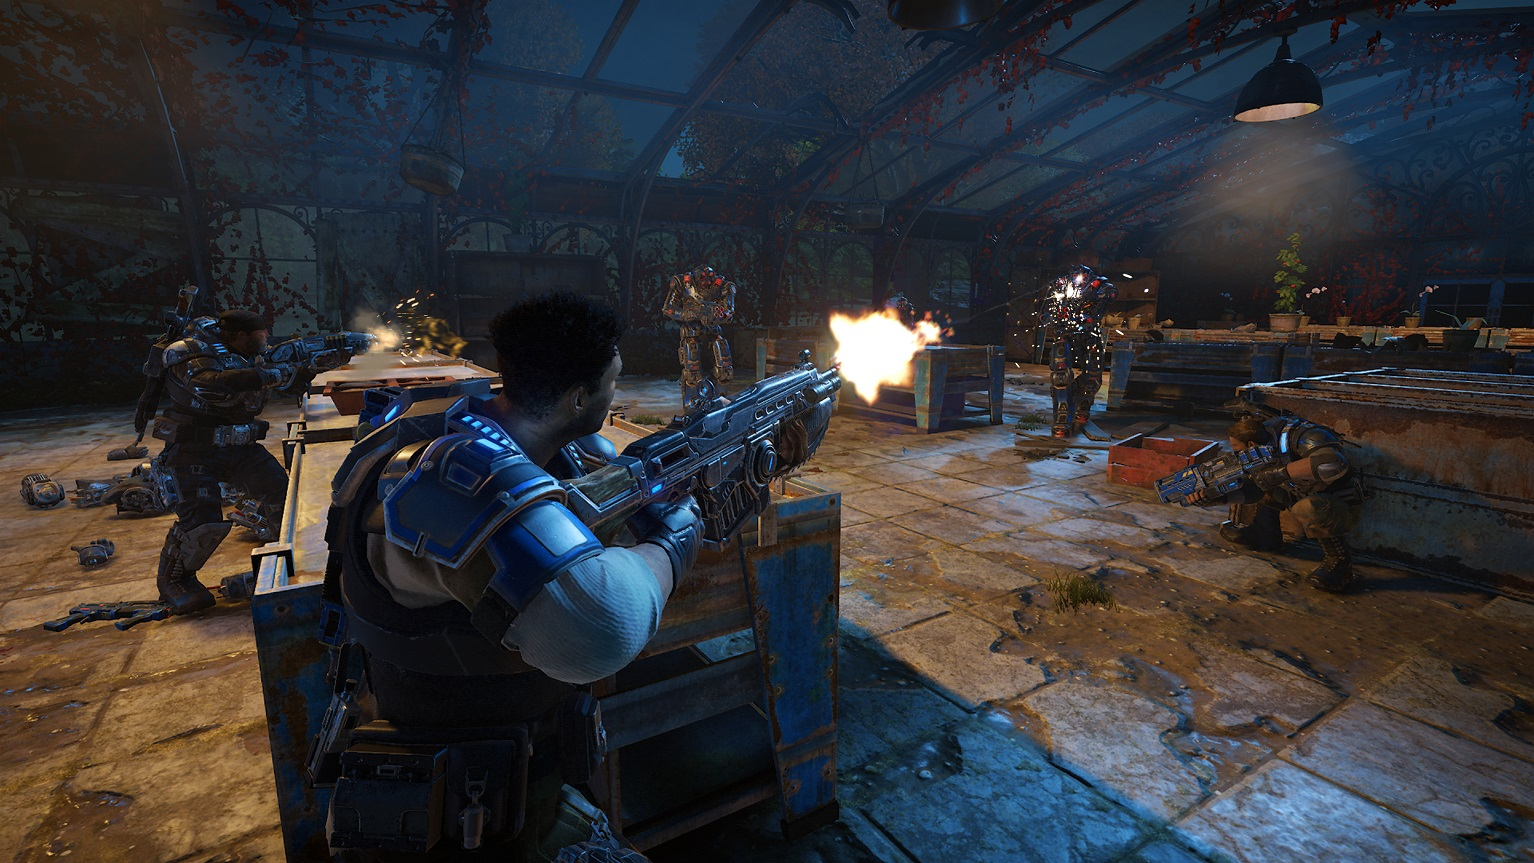
\includegraphics[width=0.21\linewidth]{figures/geow.jpg}
			}
			\subfigure[Ratatouille]{
				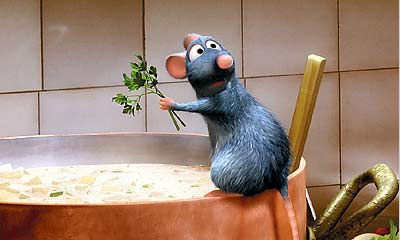
\includegraphics[width=0.20\linewidth]{figures/Ratatouille.jpg}
			}
			\subfigure[The lord of the rings]{
				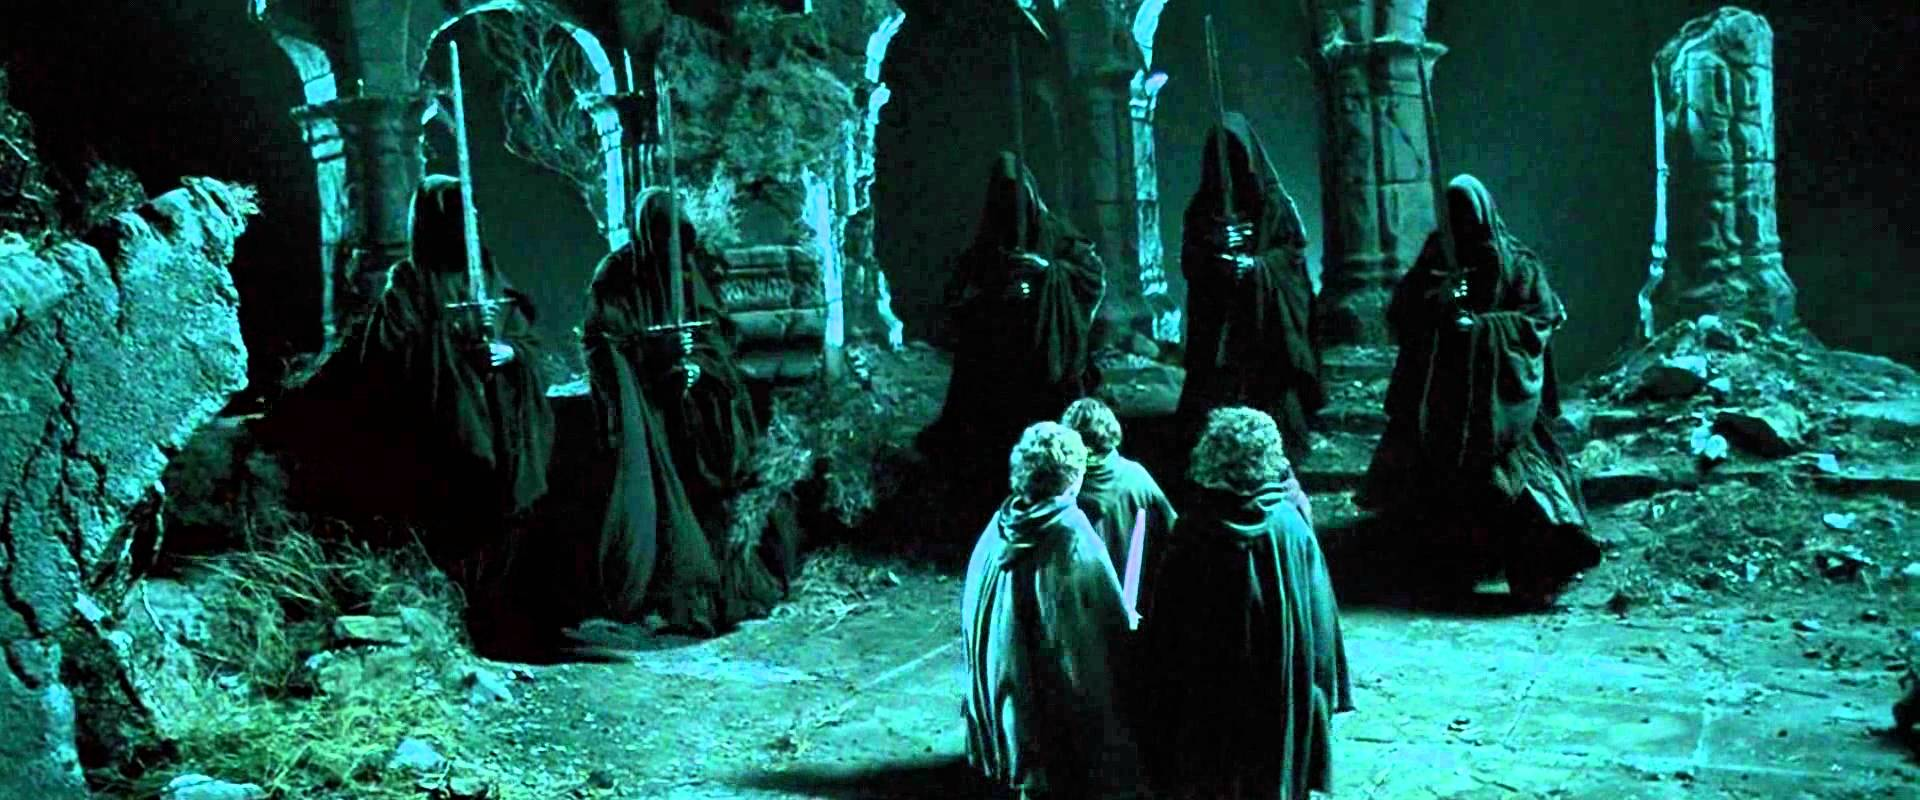
\includegraphics[width=0.29\linewidth]{figures/lotr.jpg}
			}		
		\end{figure}
	  \item My firsts...
		  \begin{figure}
			\centering
			\subfigure[First Computer (Commodore 64)]{
				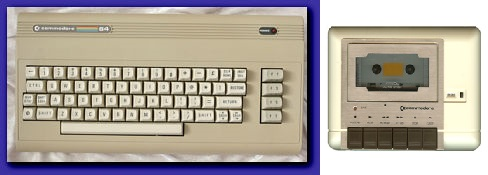
\includegraphics[height=0.2\textheight]{figures/commodore.jpg}
			}
			\subfigure[First IBM compatiable PC (80286)]{
				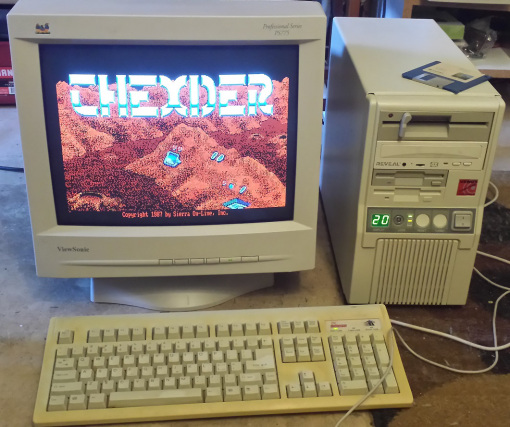
\includegraphics[height=0.2\textheight]{figures/PC286.jpg}
			}
			\subfigure[First Console (Atari 2600)]{
				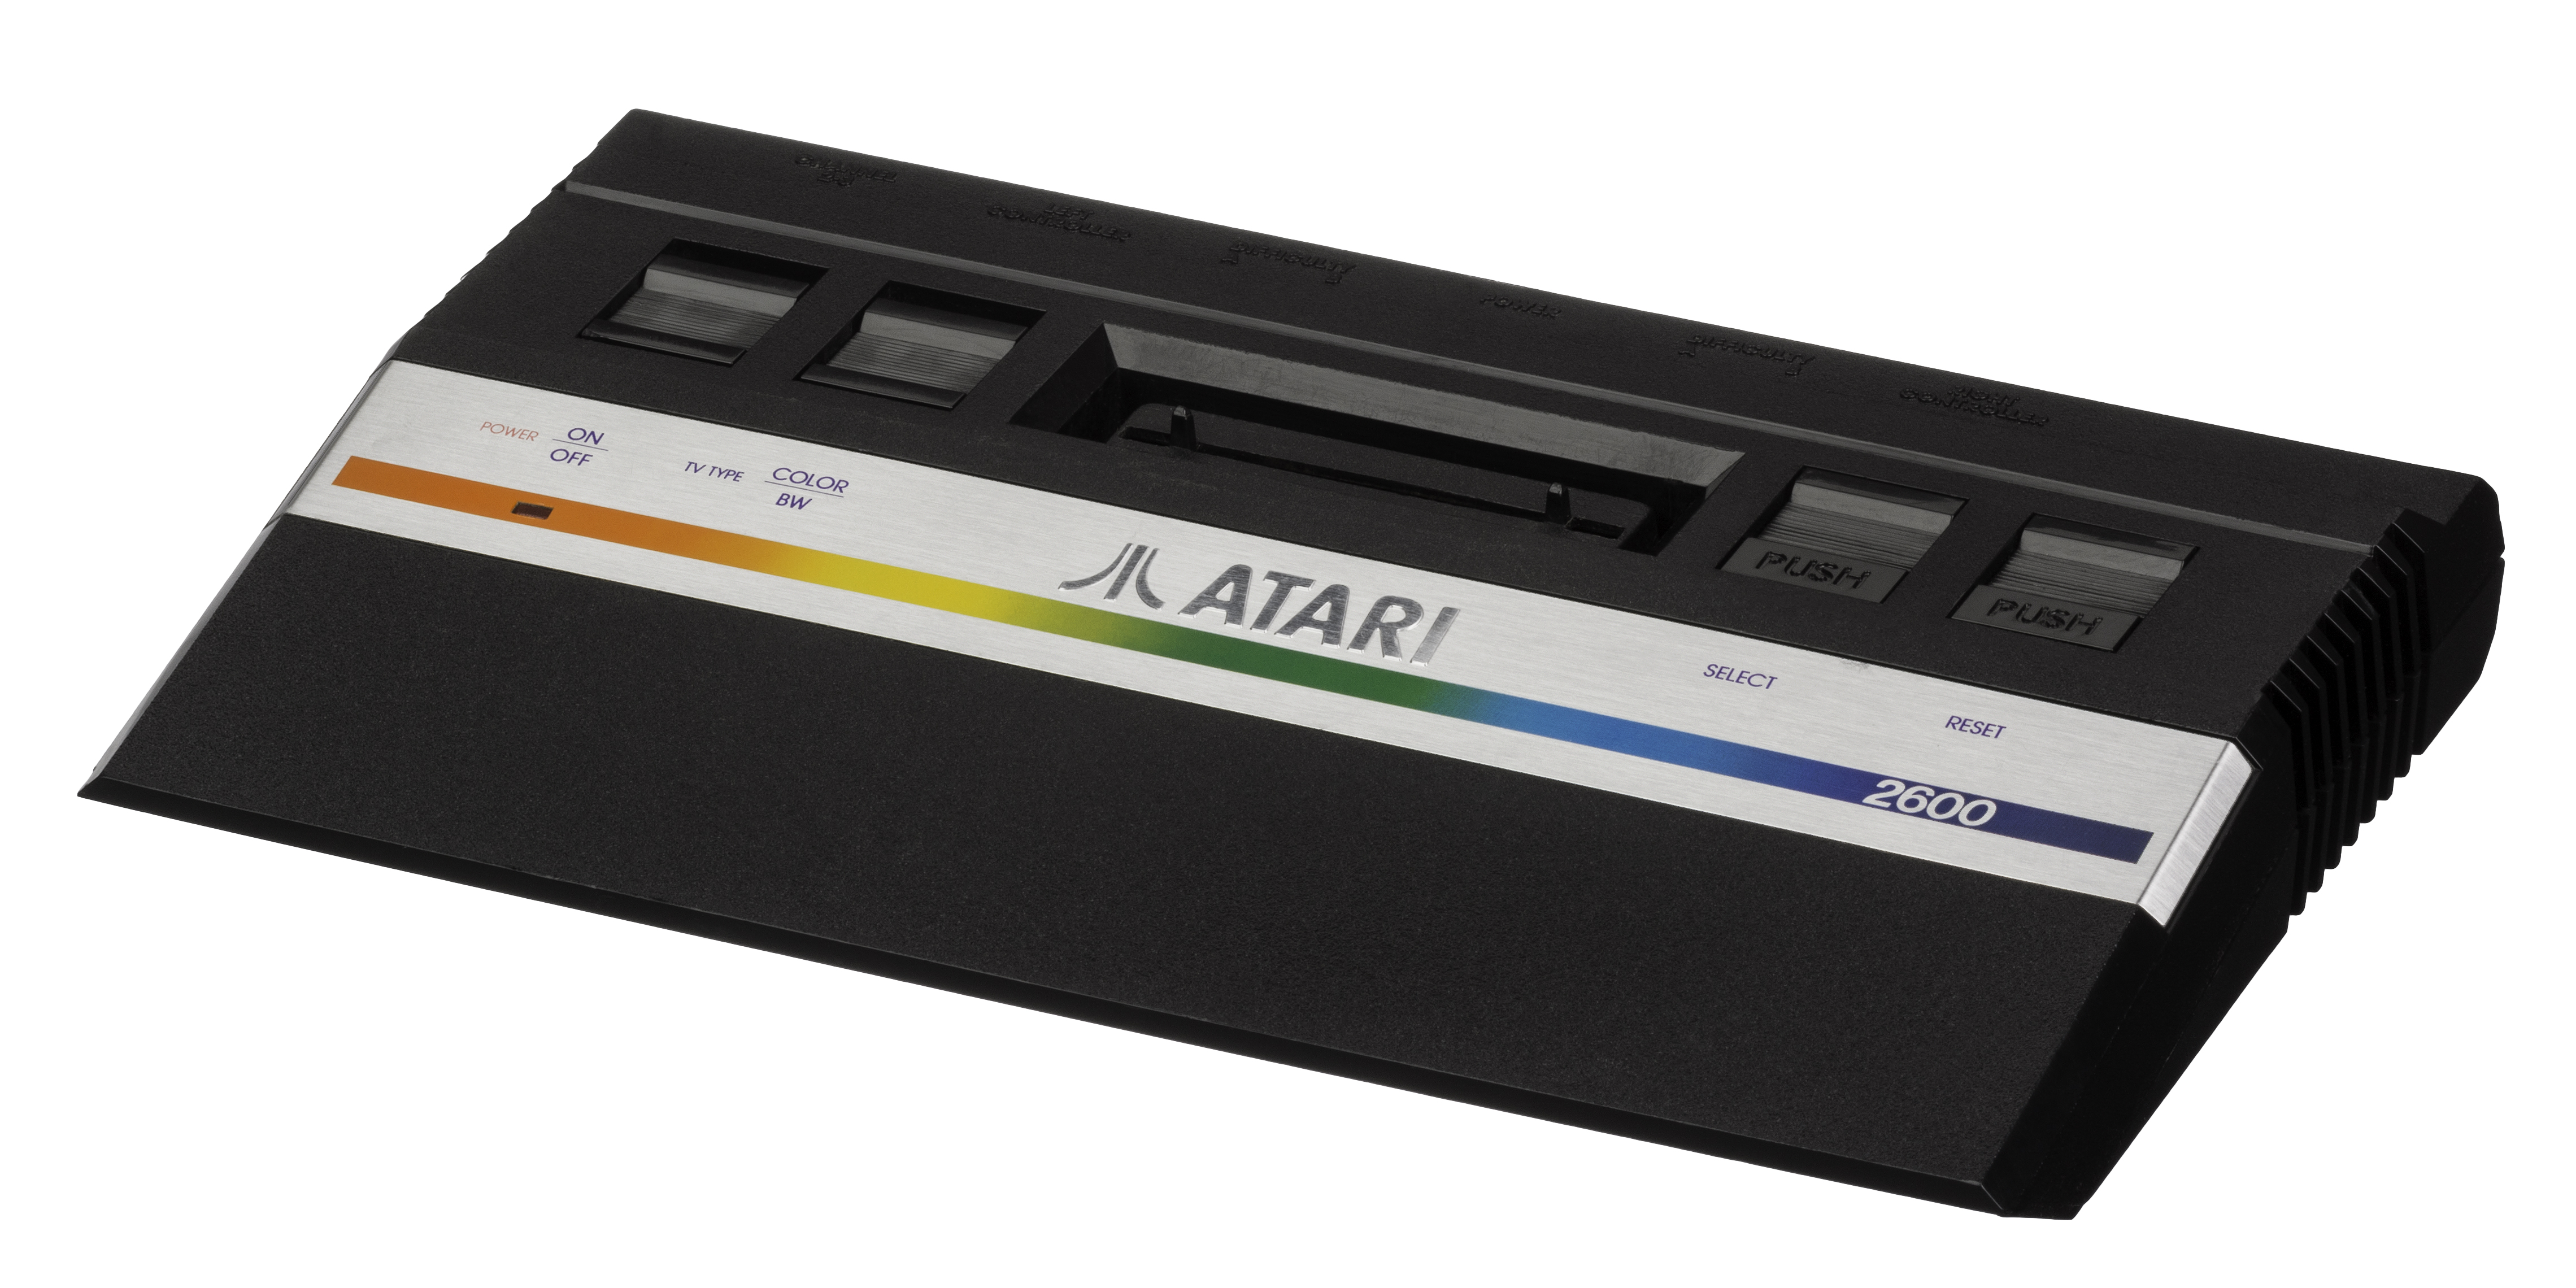
\includegraphics[height=0.15\textheight]{figures/atari2600.jpg}
			}
       	  \end{figure} 
	\end{itemize}
\end{frame}


\section{Master Thesis: Real-Time Stream Surface Computation and Rendering}

\begin{frame}{Outline}
	\tableofcontents[
	currentsection,currentsubsection,hideothersubsections
	]
\end{frame}

\begin{frame}{Real-Time Stream Surface Computation and Rendering}
	\begin{figure}
		\centering
		\subfigure[Wind Tunnel]{
			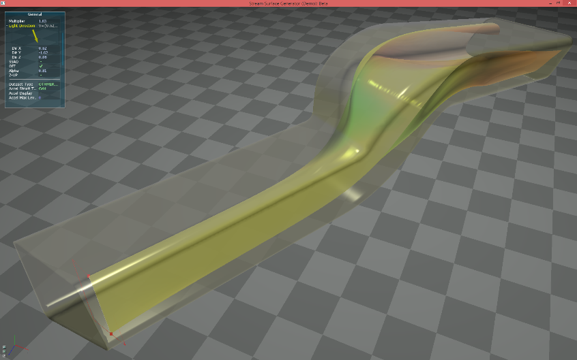
\includegraphics[height=0.3\textheight]{figures/thesis_result0}
		}
		\subfigure[Car]{
			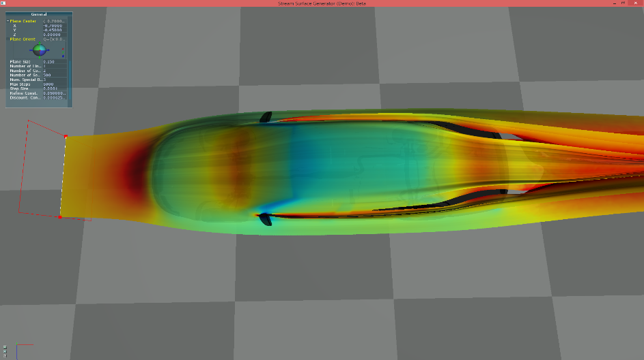
\includegraphics[height=0.3\textheight]{figures/thesis_result1}
		}\\
		\subfigure[Tethrahedradecal]{
			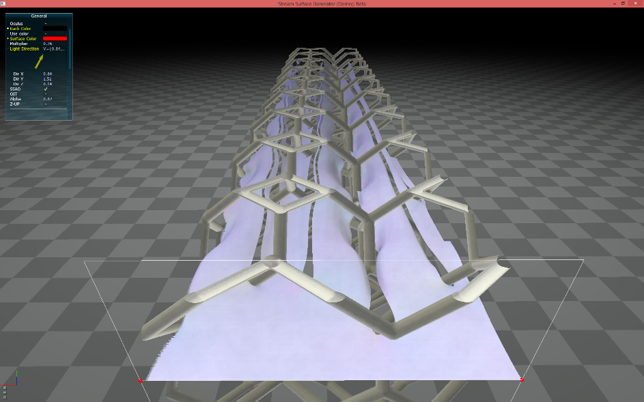
\includegraphics[height=0.3\textheight]{figures/thesis_result2}
		}
		\subfigure[Telescope]{
			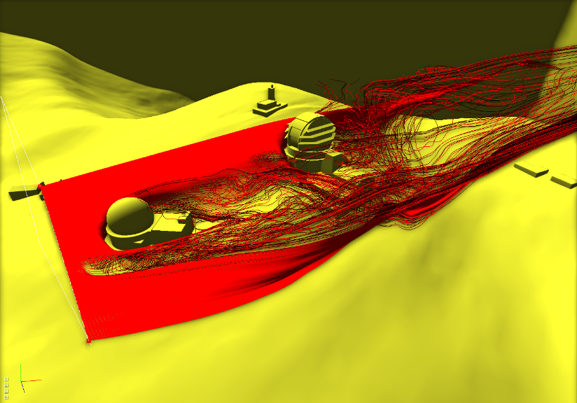
\includegraphics[height=0.3\textheight]{figures/thesis_result3}
		}
		\caption{
			Final results of this master thesis.
		}
	\end{figure}
\end{frame}

\begin{frame}{Motivation}
	\begin{itemize}
		\item \textbf{Goal}: Use virtual reality to help engineers getting a better \textbf{understanding} of simulations, make \textbf{investigation} in flow field features easier.
		\item Virtual reality applications demands 75-140 frames per second scene update and rendering to reduce \textbf{latency}.
		\item \textbf{Initial motivation}:\\
		  -- \textbf{Immersive Streamline Demo}: a demo which user could stand in a simulation model to understand flow field features by:
		  \begin{itemize}
		  	\item Prototype demo which placed the user virtually in simulation model.
		  	\item User could interact with virtual world by moving streamlines' seeding plane.
		  	\item User could walk around in the simulation model, look closer into streamlines to understand flow field's features better.
		  \end{itemize} 
	\end{itemize}
\end{frame}

\begin{frame}{Immersive Streamline Demo}

	\begin{figure}[ht!]
	\centering
	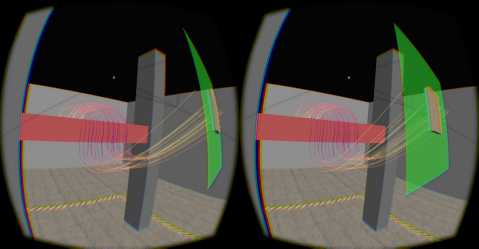
\includegraphics[width=0.9\linewidth]{./figures/vr.png}
	\caption{\textbf{Immersive Streamlines} was a prototype demo done at Fraunhofer IGD. The user is able to move inside the virtual world, interact with it, and look closely at the flow visualization results. The image shows a stereo pair, which is displayed on Oculus Rift HMD. }
	\label{fig:vr_irpv}
	
	\end{figure}
\end{frame}

\begin{frame}{Problem Definition}
	\begin{itemize}
		\item Streamline's computation was 10 frames per second (latency was very visible to user).
		\item Streamline's accuracy was not high enough (straight lines in streamlines are visible in the screenshot).
		\item Stream surfaces can provide more information about flow fields features.
		\item So, we defined \textbf{Parallel Stream Surface Computation and Rendering} master thesis to solve these problems.		
	\end{itemize}
\end{frame}

\begin{frame}{Main Contributions}
	\begin{itemize}
		\item \textbf{Contribution 1}: Using heterogeneous computing:\\
  		  -- Scale streamline computation on all capable devices.\\
		  -- Scale rendering on all graphic processing units.\\
		\item \textbf{Contribution 2}: Investigation techniques from ray tracing field for application in accurate streamline computation:\\
		  -- Using acceleration structures\\
		  -- Using ray-packing\\
	\end{itemize}
\end{frame}

\begin{frame}{Benefits}
	
	\begin{itemize}
		\item Accurate streamline computation method (using \textbf{Runge-Kutta} integration method).
		\item \textbf{Adaptive Runge-Kutta} integration method to adapt steps to maximum integration error.
		\item Heterogeneous stream surface computation.
		\item Multi GPU stream surface computation and result 
	\end{itemize}
	\textbf{}
	
\end{frame}

\begin{frame}{Related Works}
	\begin{itemize}
		\item Parallel stream surface computation for large data sets \cite{CampPaper}.\\
		proposed a distributed stream surface computation system.\\
		-- \textbf{My method is not distributed but uses all available computation devices.}
		\item Interactive Streak Surface Visualization on the GPU \cite{BurgerStreakSurface}.\\
		Bue+09 samples the simulation mesh on a regular grid, then compute the streak surface.\\
		-- \textbf{Reduces accuracy, ignores a lot of information exist in simulation mesh by sampling it on a regular grid.}
	\end{itemize}
\end{frame}

\begin{frame}{Related Works}
	\begin{itemize}
		\item Interactive particle tracing for the exploration of flow fields in virtual environments \cite{Schirski:50085}.\\
		Sch08 uses the neighboring graph instead of acceleration
		structure on GPU.\\
		-- \textbf{step size needed to be small enough.}
		\item Fast, Memory-Efficient Cell Location in Unstructured Grids for
		Visualization \cite{GarthPaper}.\\
		introduces cell-tree acceleration structure use it for
		particle tracing.\\
		-- \textbf{I have evaluated more acceleration structures to classify them based on memory requirements and performance.}
	\end{itemize}
\end{frame}

\begin{frame}{Stream Surface Computation Algorithm \cite{CampPaper}}
	\begin{algorithm}[H]
		\KwData{$seeds$ list which contains all initial seeding points.}
		\KwResult{Stream Surface Points}

		\While{$seeds$ list is not empty}{
			
			\textbf{Tracing}: Trace streamlines originating from seeding points stored in $seeds$ list and make $seeds$ empty.\
			
			\textbf{Refinement}:\For{each pair of adjacent streamlines $s_1$ and $s_2$}{
		$d \gets$ \textit{Distance}($s_1$, $s_2$)\
		
				\eIf{$d \leq D_{disc}$ }{
					\textbf{Discontinuity}: The surface is discontinued in that area.
				}{
					$s_{new} \gets (s_1[0] + s_2[0]) / 2$\\			  
					add $s_{new}$ to list $seeds$.
				}
			}
		}
		\caption{Stream Surface Computation Algorithm \cite{CampPaper}.}
	\end{algorithm}
\end{frame}

\begin{frame}{Accurate Streamline Computation}
	\begin{itemize}
		\item Point-Inside-Cell checks \& interpolating results inside cells.
		\item Using \textit{adaptive Runge-Kutta} integration method (Cash-Karp).
		\item Adaptive stepping (faster and more accurate integration).
		\item Avoiding early terminations.
	\end{itemize}
    \begin{figure}
    	\centering
    	\subfigure[Euler]{
    		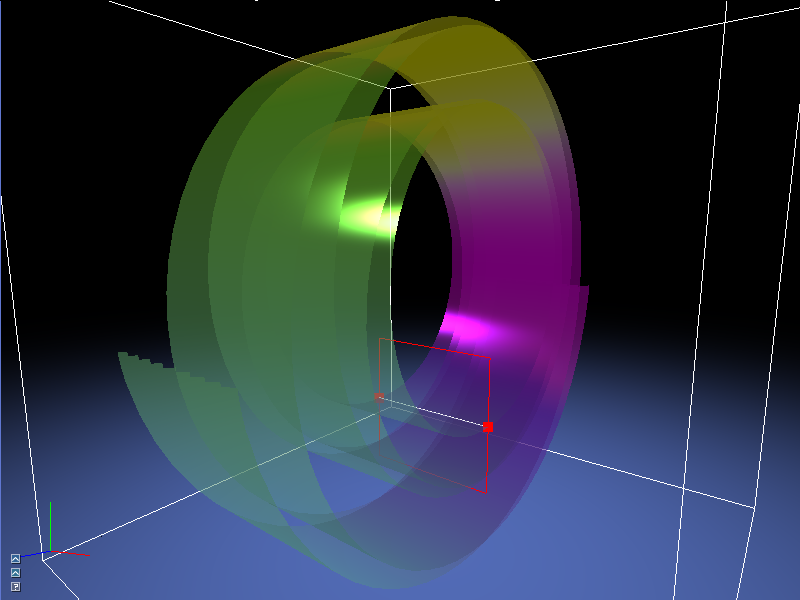
\includegraphics[width=0.4\linewidth]{figures/euler}
    	}
    	\subfigure[Cash-Karp]{
    		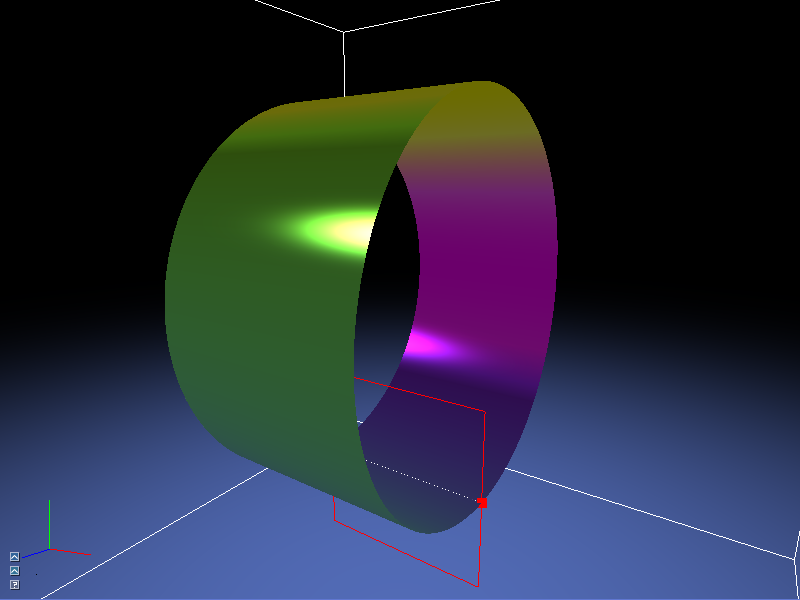
\includegraphics[width=0.4\linewidth]{figures/cashkarp}
    	}
	    \caption{Euler and Runge-Kutta integration methods in a perfect rotation around center which are integrated with the same step size.}
    \end{figure}
\end{frame}

\begin{frame}{Refinement Strategy Results}
	\begin{figure}
		\centering
		\subfigure[No Refinements]{
			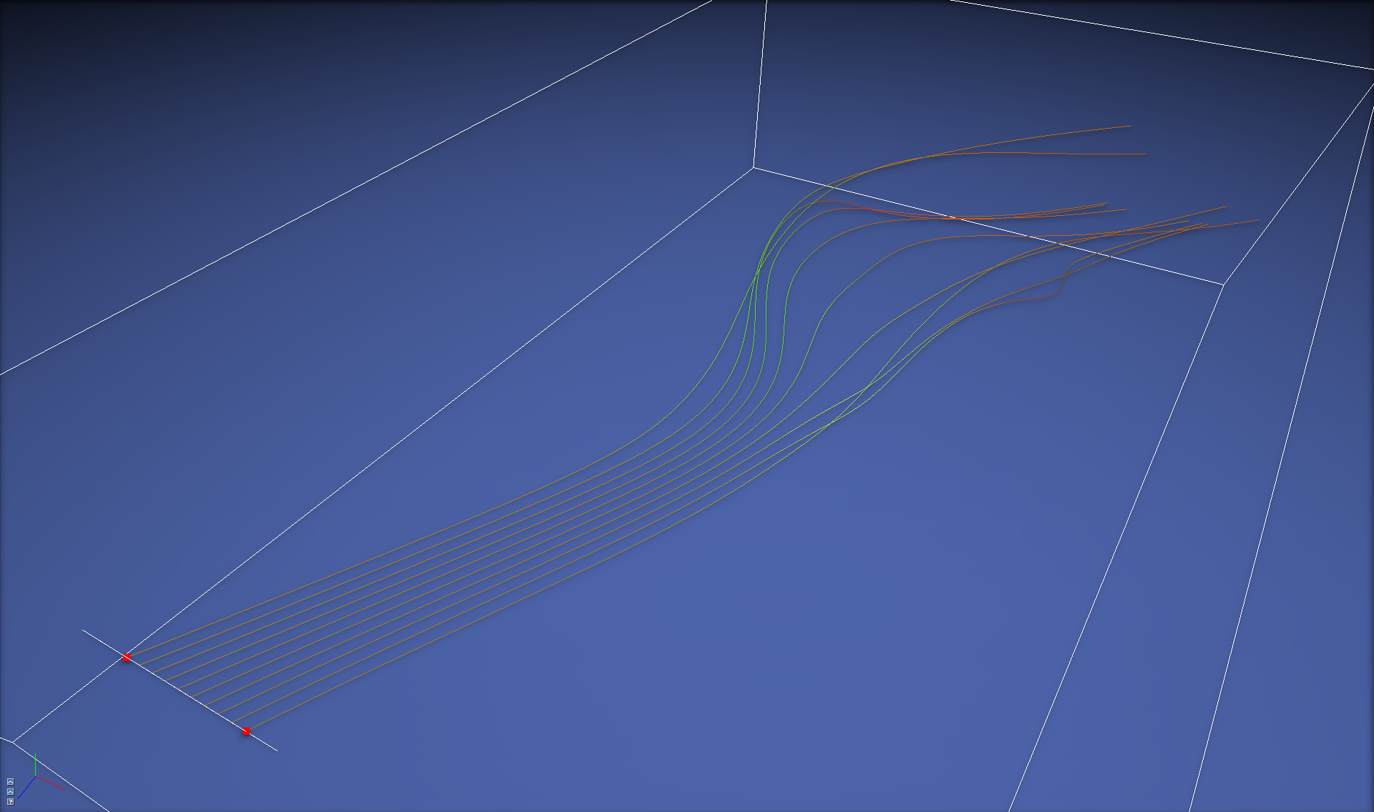
\includegraphics[width=0.3\linewidth]{figures/Refinement_0}
		}
		\subfigure[The first refinement iteration]{
			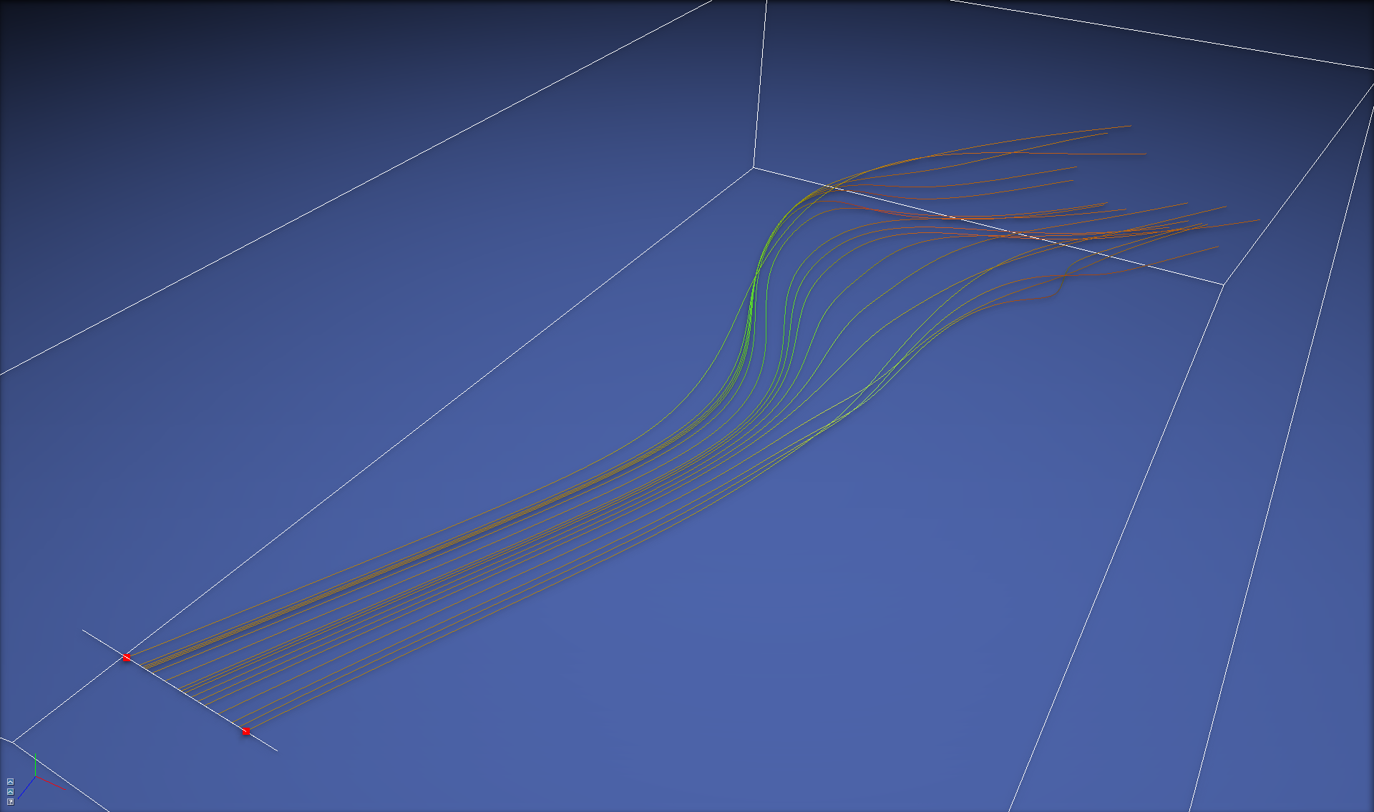
\includegraphics[width=0.3\linewidth]{figures/Refinement_1}
		}
		\subfigure[The second refinement iteration]{
			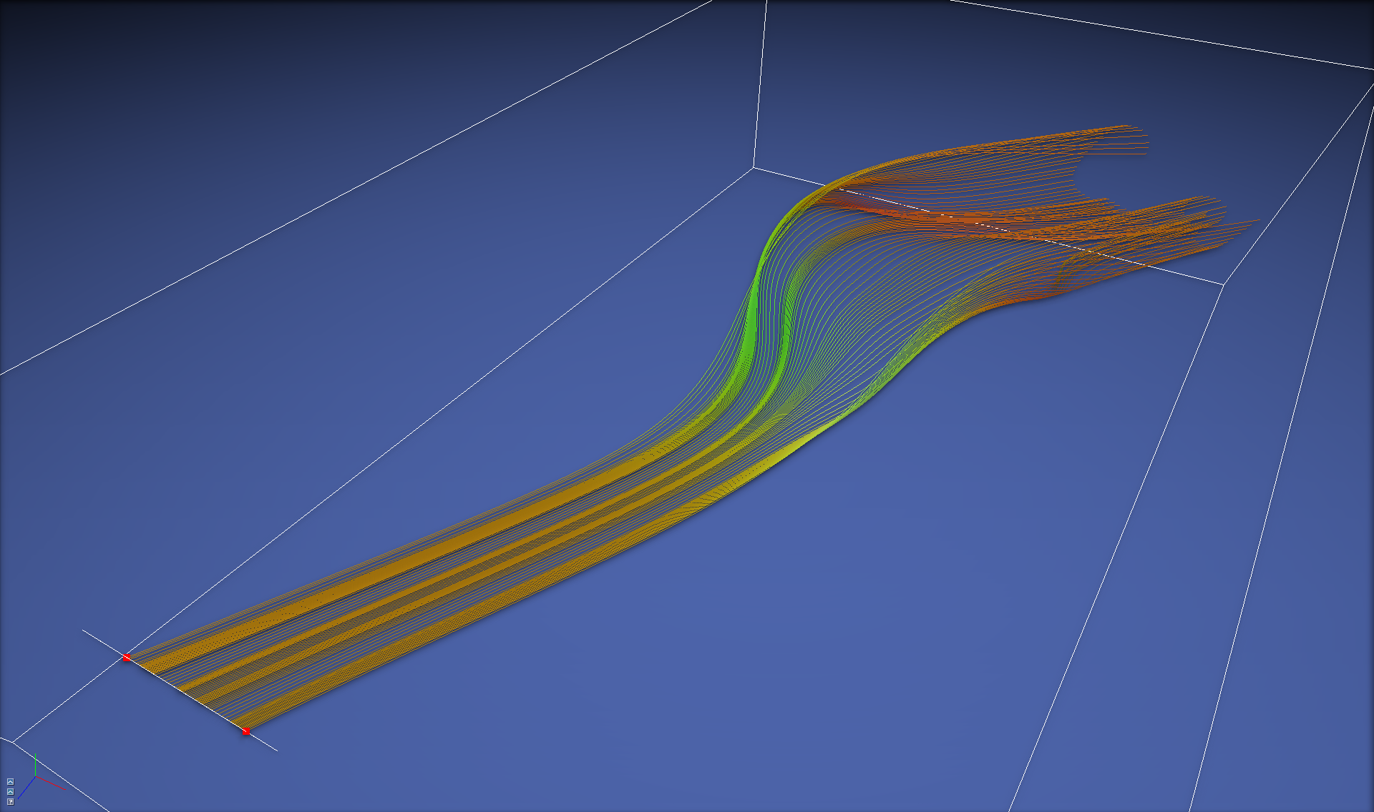
\includegraphics[width=0.3\linewidth]{figures/Refinement_2}
		}
		\caption{The result streamlines making skeleton of stream surface after 2 steps refinement.}
	\end{figure}
\end{frame}

\begin{frame}{Contrib. 1: Heterogeneous Computing Arch. (1/7)}
	\begin{figure}
		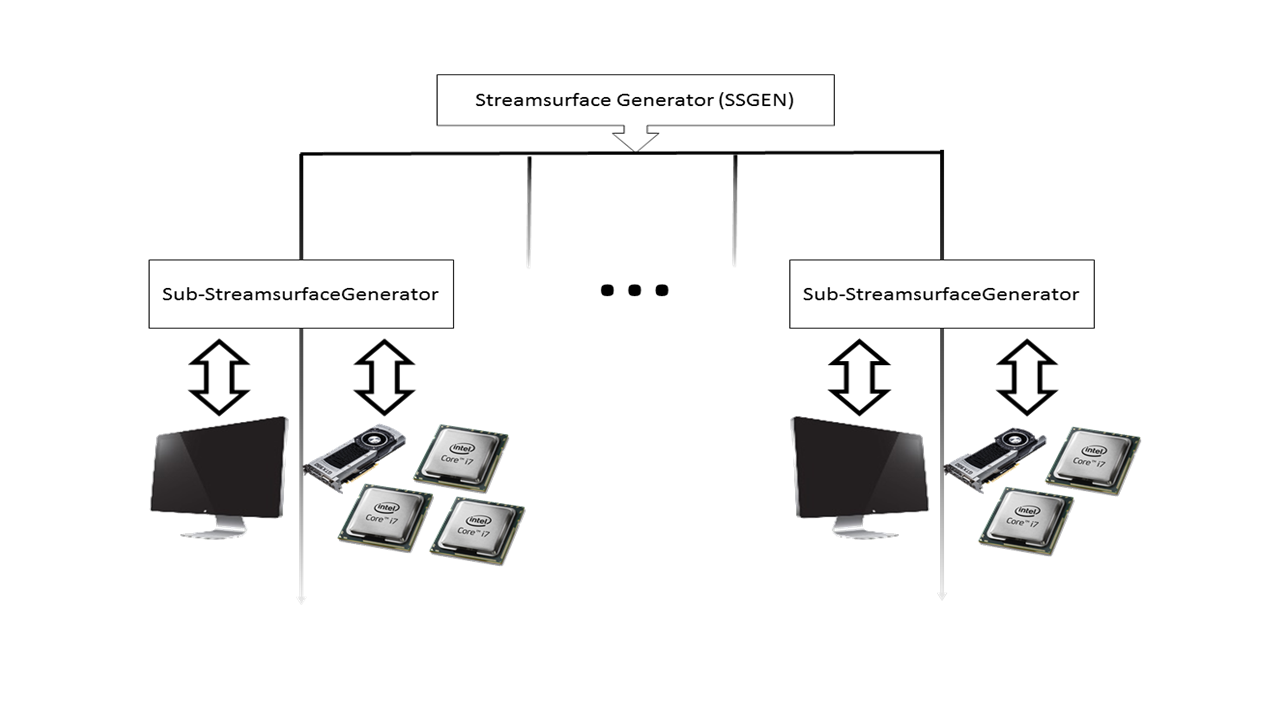
\includegraphics[width=\linewidth]{figures/MAarch1.PNG}
	\end{figure}
\end{frame}

\begin{frame}{Contrib. 1: Heterogeneous Computing Arch. (2/7)}
	\begin{figure}
		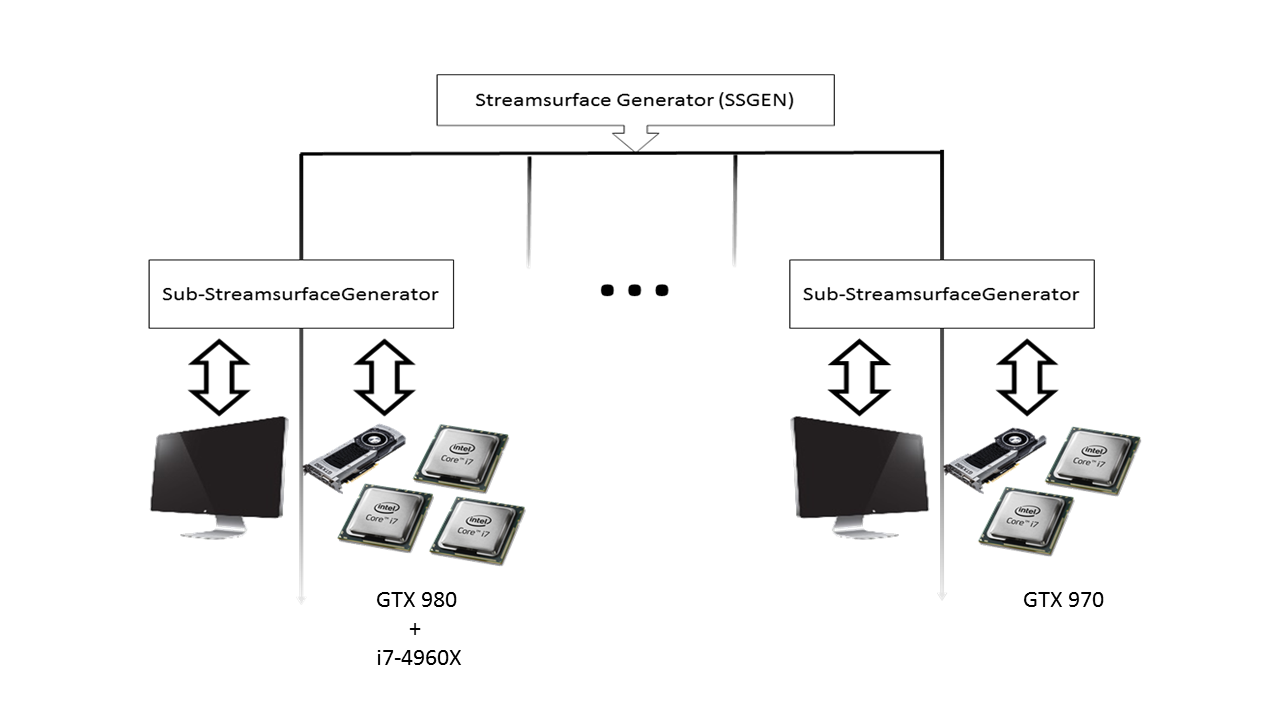
\includegraphics[width=\linewidth]{figures/MAarch2.PNG}
	\end{figure}
\end{frame}

\begin{frame}{Contrib. 1: Heterogeneous Computing Arch. (3/7)}
	\begin{figure}
		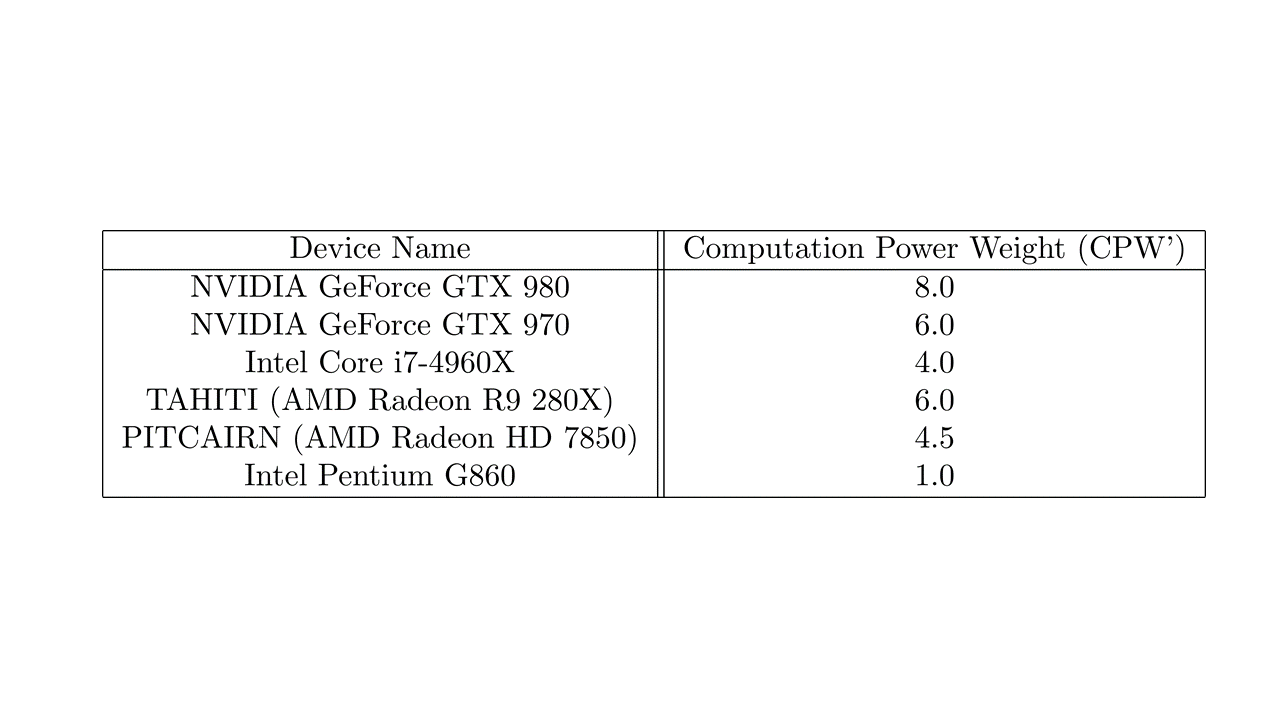
\includegraphics[width=\linewidth]{figures/MAarch3.PNG}
	\end{figure}
\end{frame}

\begin{frame}{Contrib. 1: Heterogeneous Computing Arch. (4/7)}
	\begin{figure}
		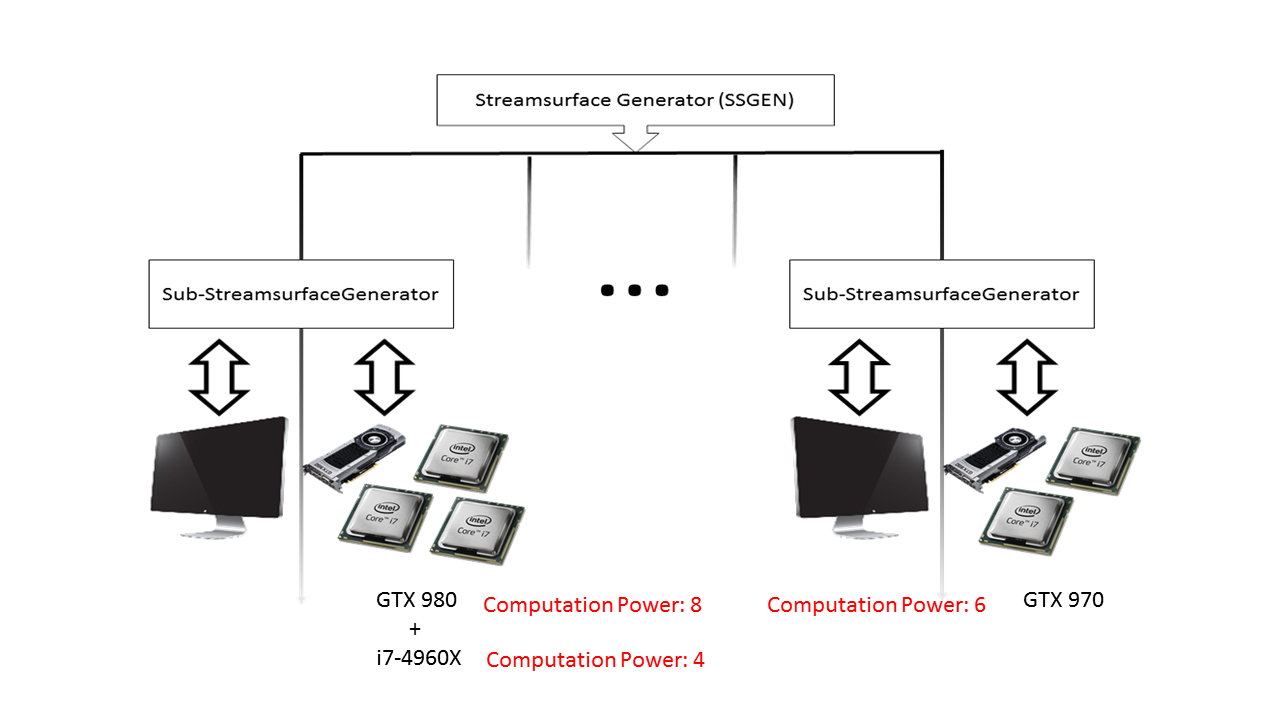
\includegraphics[width=\linewidth]{figures/MAarch4.PNG}
	\end{figure}
\end{frame}

\begin{frame}{Contrib. 1: Heterogeneous Computing Arch. (5/7)}
	\begin{figure}
		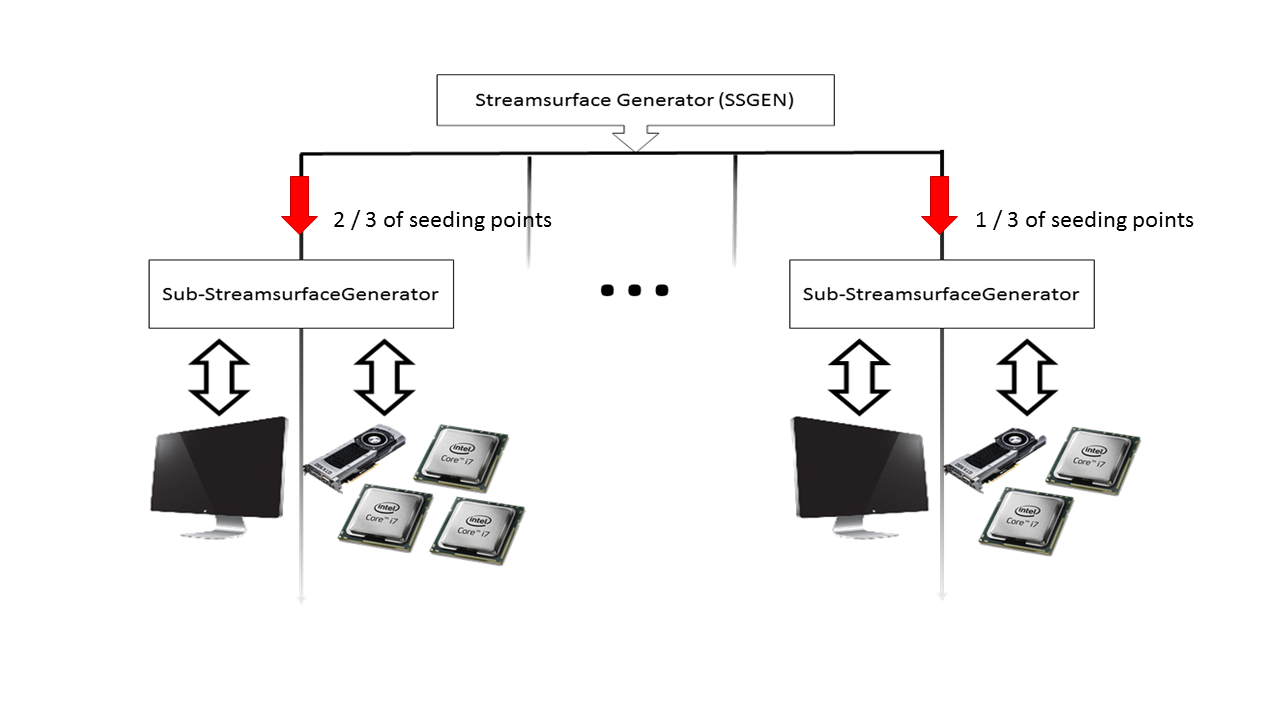
\includegraphics[width=\linewidth]{figures/MAarch5.PNG}
	\end{figure}
\end{frame}

\begin{frame}{Contrib. 1: Heterogeneous Computing Arch. (6/7)}
	\begin{figure}
		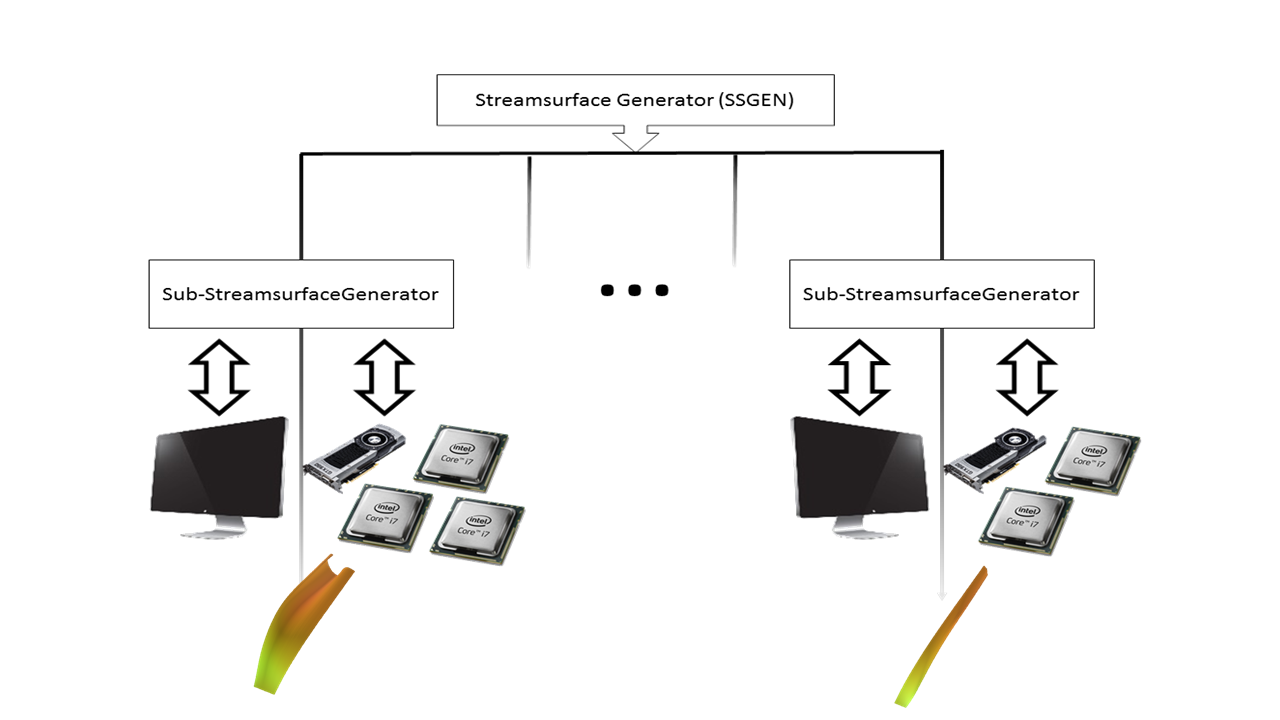
\includegraphics[width=\linewidth]{figures/MAarch6.PNG}
	\end{figure}
\end{frame}

\begin{frame}{Contrib. 1: Heterogeneous Computing Arch. (7/7)}
	\begin{figure}
		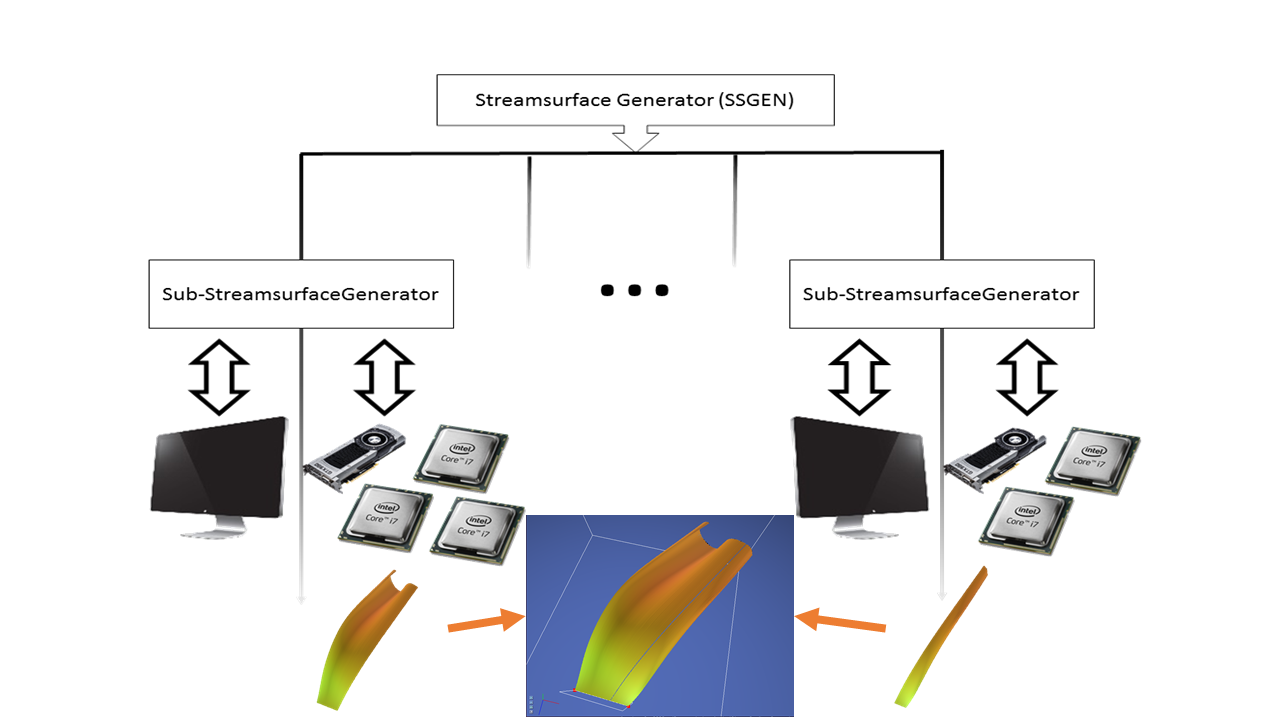
\includegraphics[width=\linewidth]{figures/MAarch7.PNG}
	\end{figure}
\end{frame}

\begin{frame}{Multi GPU Rendering}
	\begin{itemize}
		\item Compositing screen cpace ambient occlusion results
		\begin{figure}
			\centering
			\subfigure[GPU \#0]{
				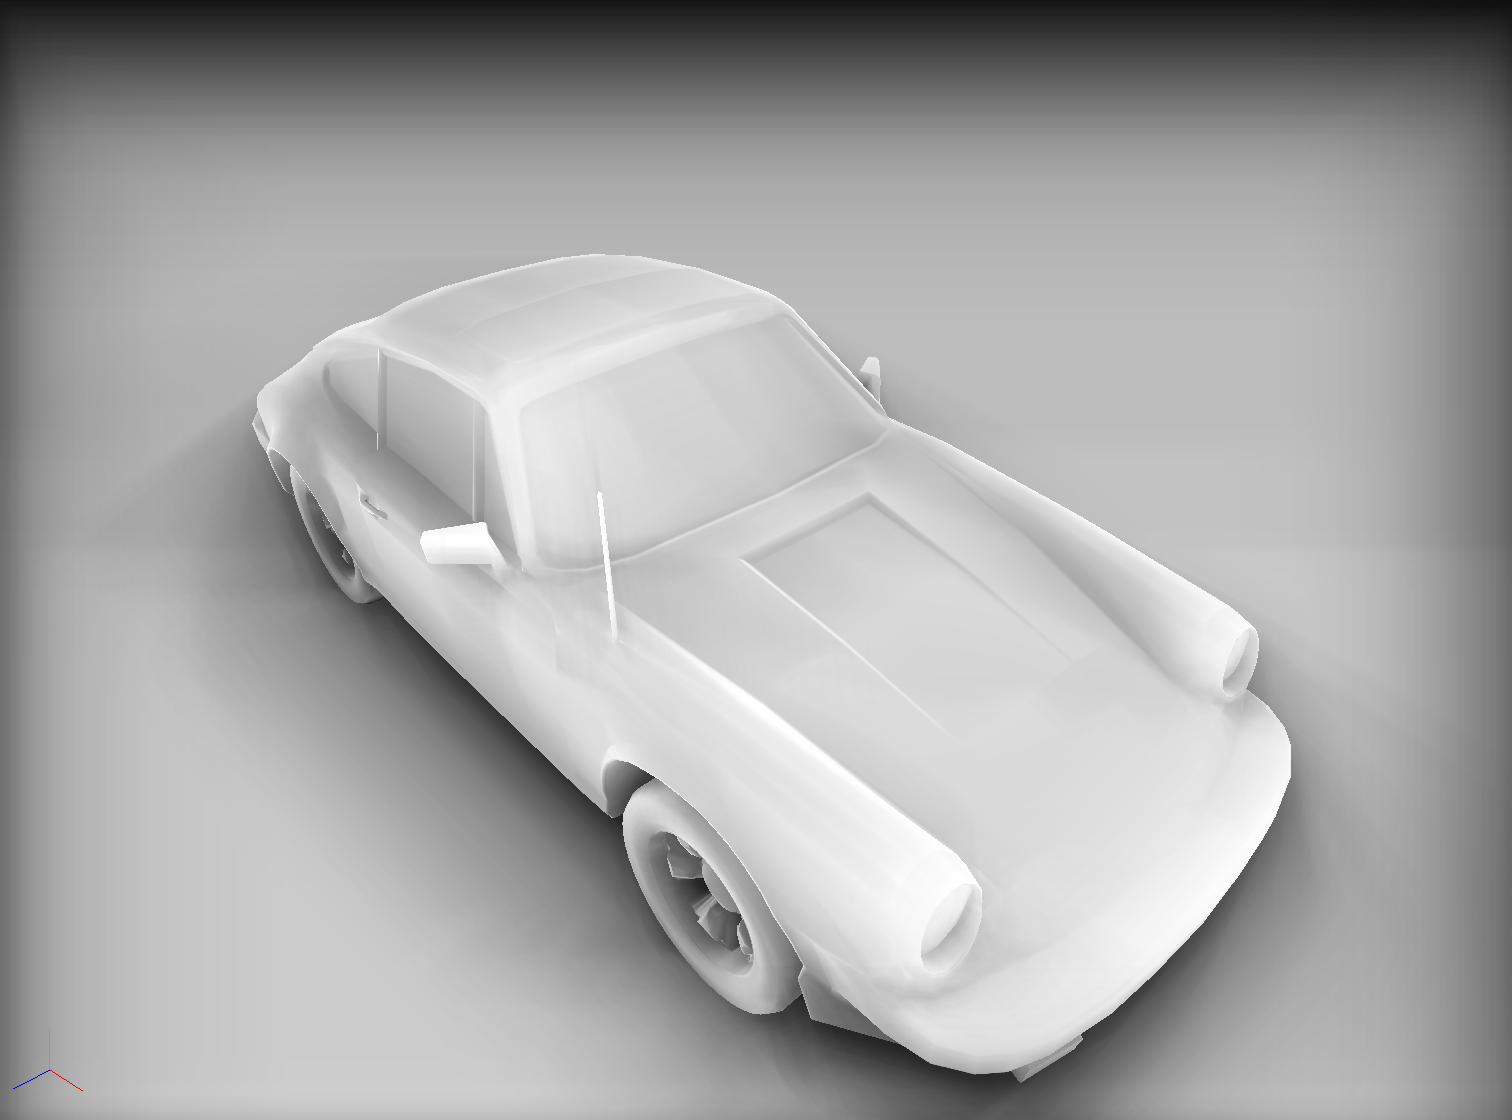
\includegraphics[height=0.25\textheight]{figures/SSAO_GPU0}
			}
			\subfigure[GPU \#1]{
				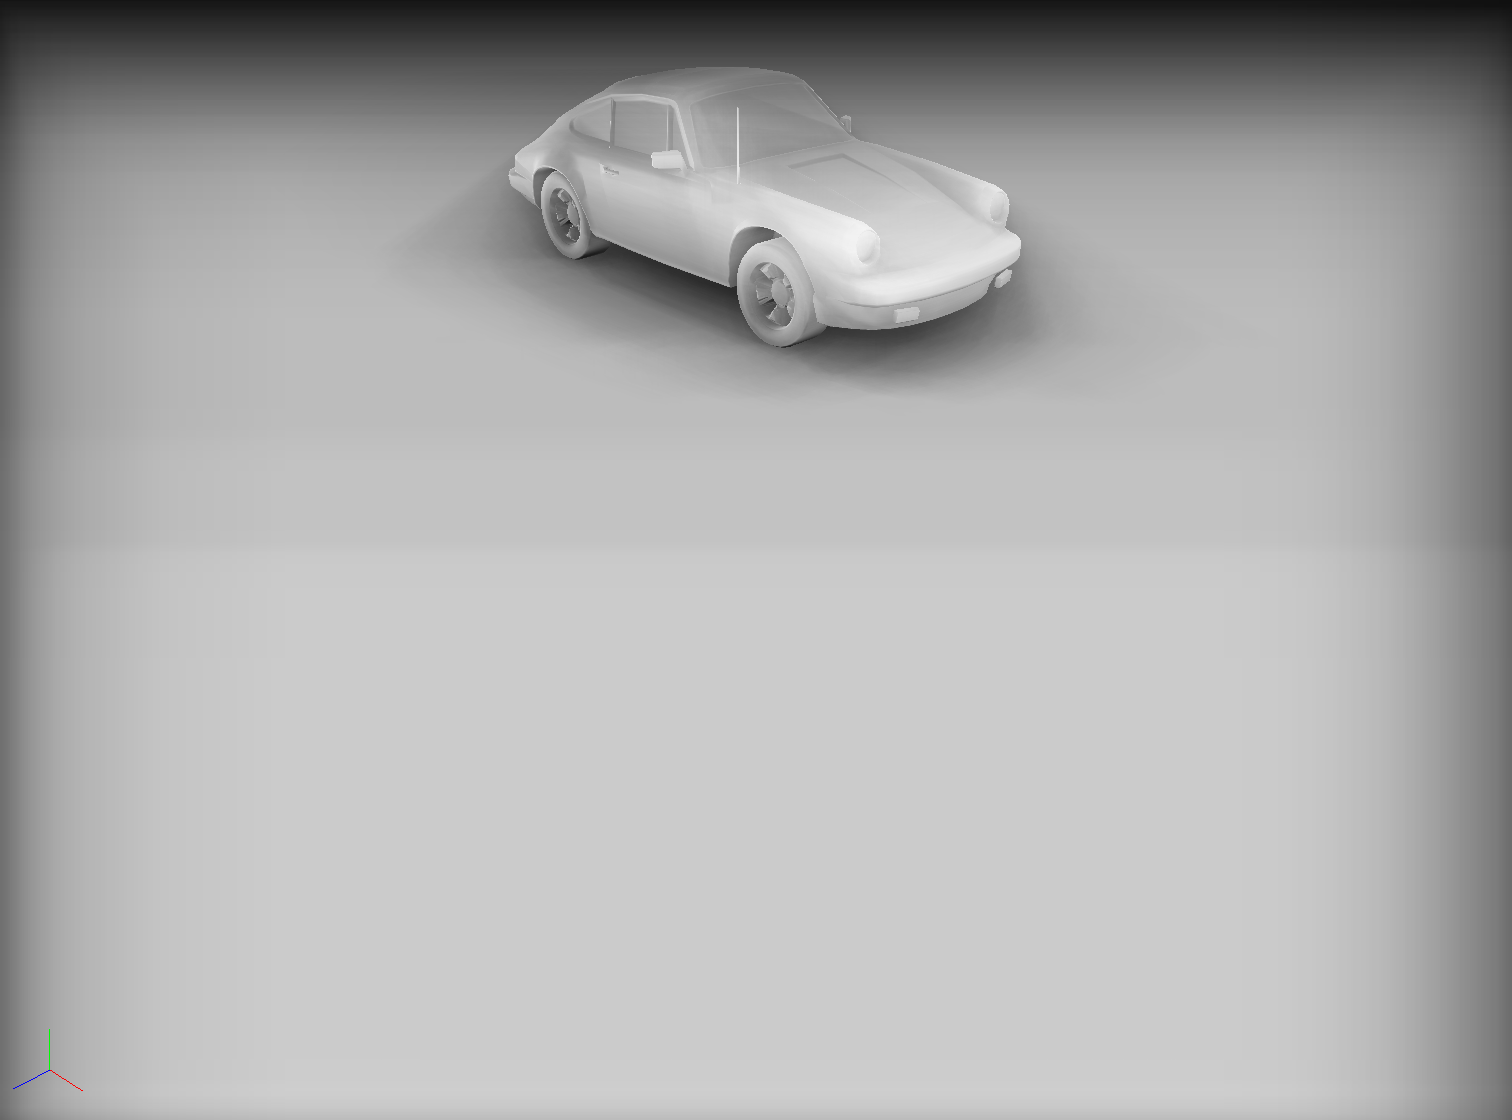
\includegraphics[height=0.25\textheight]{figures/SSAO_GPU1}
			}
			\subfigure[Composited]{
				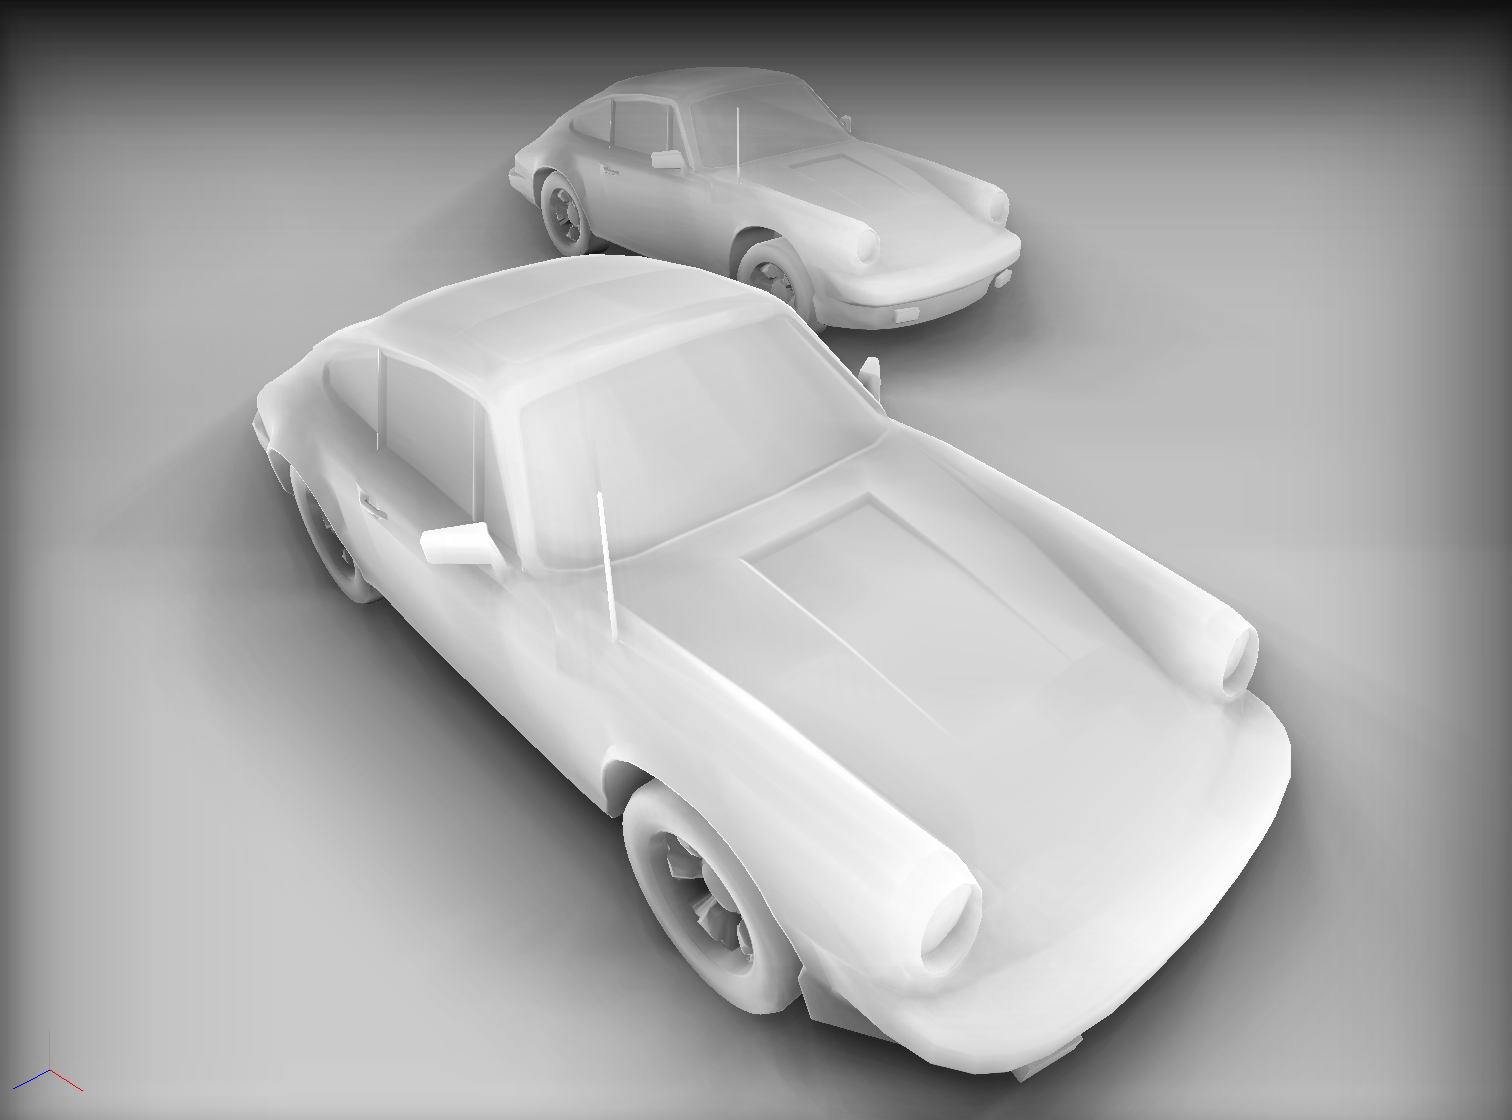
\includegraphics[height=0.25\textheight]{figures/SSAO_Combined}
			}
		\end{figure}
	
		\item Compositing order independence transparency results
		\begin{figure}
			\centering
			\subfigure[GPU \#0]{
				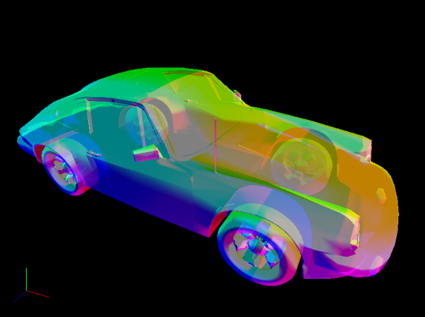
\includegraphics[height=0.25\textheight]{figures/OIT_GPU0}
			}
			\subfigure[GPU \#1]{
				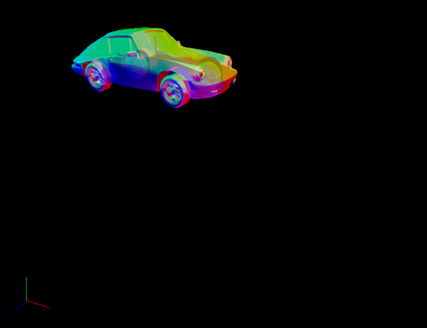
\includegraphics[height=0.25\textheight]{figures/OIT_GPU1}
			}
			\subfigure[Composited]{
				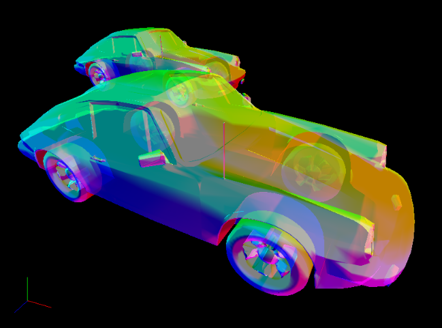
\includegraphics[height=0.25\textheight]{figures/OIT_Composited}
			}
		\end{figure}
	\end{itemize}
\end{frame}

\begin{frame}{Heterogeneous Computing Results}
	\begin{itemize}
		\item Measured parameters:
		\begin{itemize}
			\item \textbf{Computations per second}: It shows how many times the stream surface can be computed in every second. The unit is number of computation times per second.
			\item \textbf{Number of seeding points}: Total number of seeding points for producing the final stream surface.
		\end{itemize}
	\end{itemize}
\end{frame}

\begin{frame}{}
	\centering
	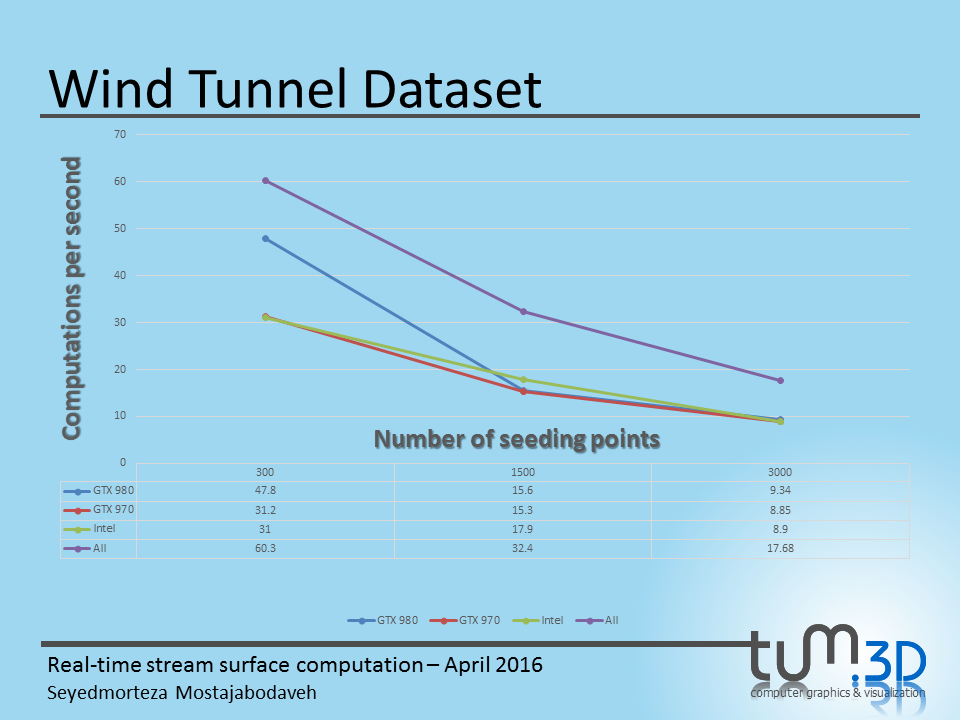
\includegraphics[height=\textheight]{figures/Slide19}
\end{frame}

\begin{frame}{}
	\centering
	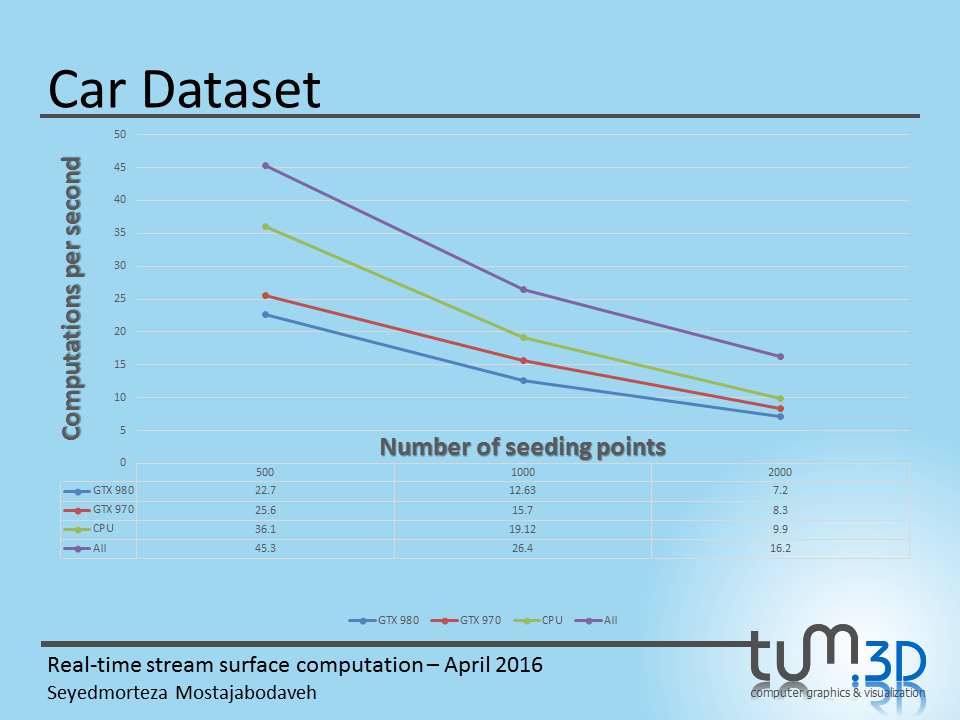
\includegraphics[height=\textheight]{figures/Slide20}
\end{frame}

\begin{frame}{Heterogeneous Computing Results Conclusions}
	\begin{itemize}
		\item As expected, the streamline computation is being scaled on all available computation devices.
		\item Using both GPUS and CPU, the computation performance is doubled.
		\item Limiting factors:\\
			\begin{itemize}
				\item OpenGL operations cannot be parallelized.
				\item Synchronization of threads are a overhead.
				\item \textbf{Dynamic task scheduling} could be a better approach.				
			\end{itemize}
		\item There is an overhead for initializing computations on multiple devices.
	\end{itemize}
\end{frame}

\begin{frame}{Acceleration Structures}
	
	\begin{columns}
		\begin{column}{.49\textwidth}
			\begin{itemize}
				\item Grid
				\item Kd-tree
				\item Bounding Volume Hierarchy (BVH)
				\item Cell-tree \cite{GarthPaper}
			\end{itemize}
		\end{column}
		
		\begin{column}{.49\textwidth}
			\begin{figure}[!ht]
				\centering
				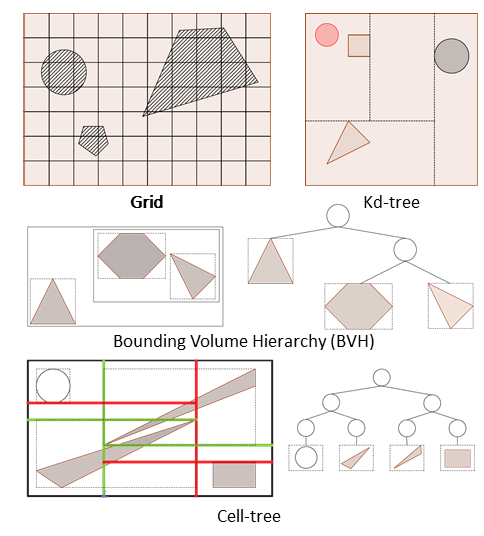
\includegraphics[width=1.0\linewidth]{figures/accelstructs}
			\end{figure}
		\end{column}
	\end{columns}
\end{frame}

\begin{frame}{Why Acceleration Structures?}
	\begin{itemize}
		\item Accelerating cell look up for faster streamline computation.
		\item Ray tracing uses acceleration structures to find \textbf{nearest intersection point} in contrast to streamline computation which uses it to \textbf{sample result in a specific point}.
		\item Differences:
		    \begin{itemize}
		    	\item In streamline computation instead of \textit{Surface Area} Heuristics, textit{Volume} Heuristics should be used.
		    	\item \textit{Traversal algorithms} for space partitioning cases does not need \textit{stack}.
		    	\item Hierarchy traversal algorithms need a greedy method to prefer one child to other one during traversal.
		    \end{itemize}
		
	\end{itemize}
\end{frame}

\begin{frame}{Contrib. 2: Using Acceleration Structures for Streamline Computation Evaluations}
	\begin{itemize}
		\item Measured parameters:
			 \begin{itemize}
			 	\item \textbf{Avg. checks per traverse}: Average number of bounding box or point-inside-cell tests done to find the cell surrounding the sample point.
			 	\item \textbf{Size in memory}: Size of the constructed acceleration structured in memory.
			 \end{itemize}
	\end{itemize}
\end{frame}

\begin{frame}{}
	\centering
	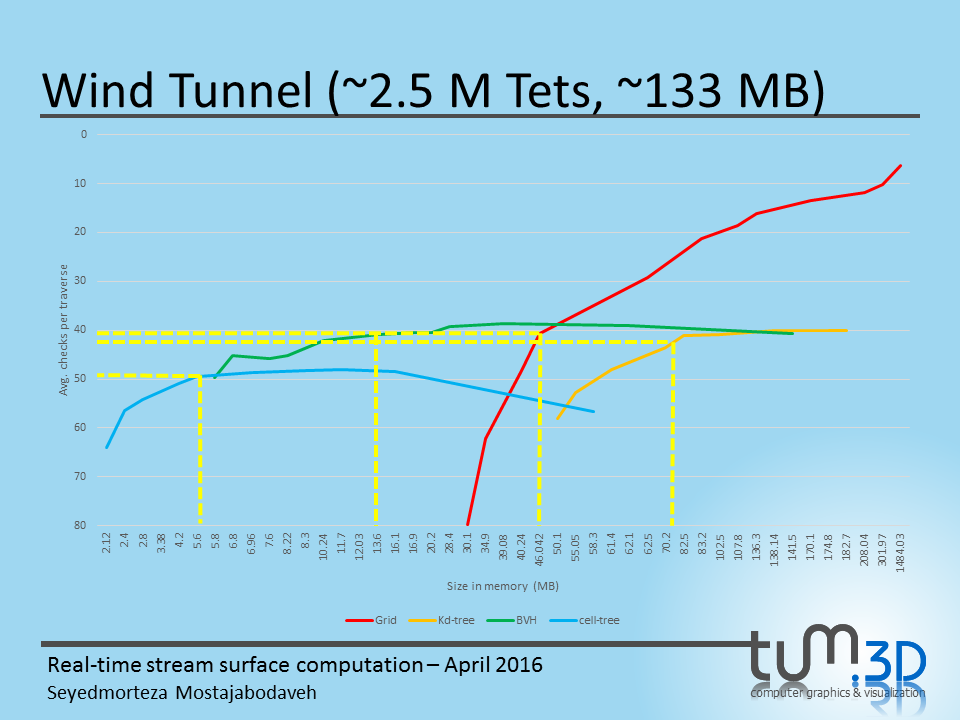
\includegraphics[height=\textheight]{figures/Slide23}
\end{frame}

\begin{frame}{}
	\centering
	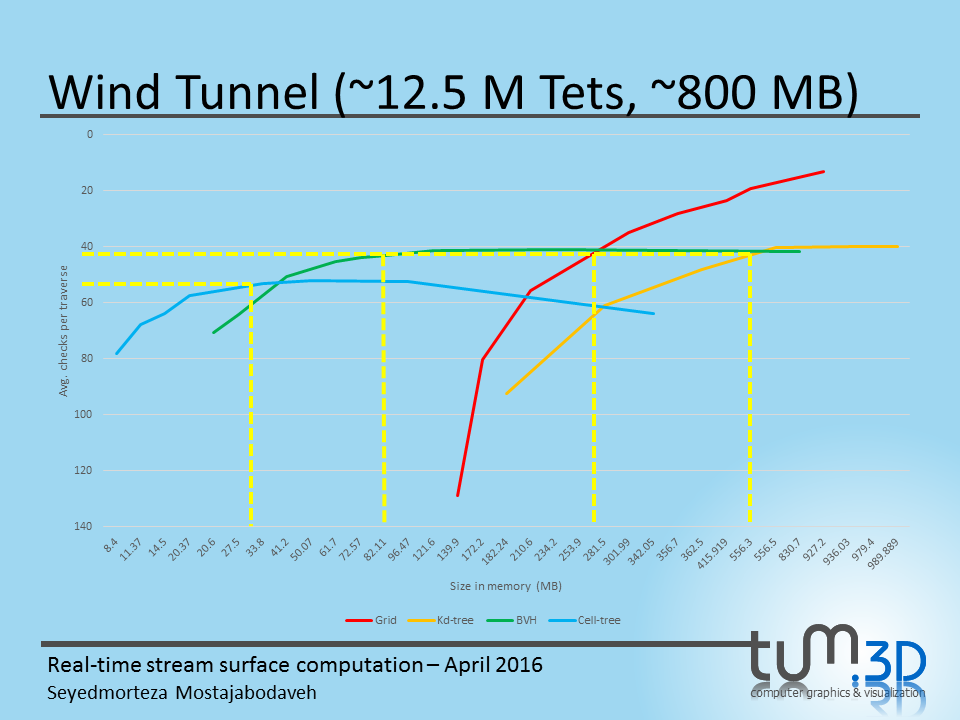
\includegraphics[height=\textheight]{figures/Slide25}
\end{frame}

\begin{frame}{}
	\centering
	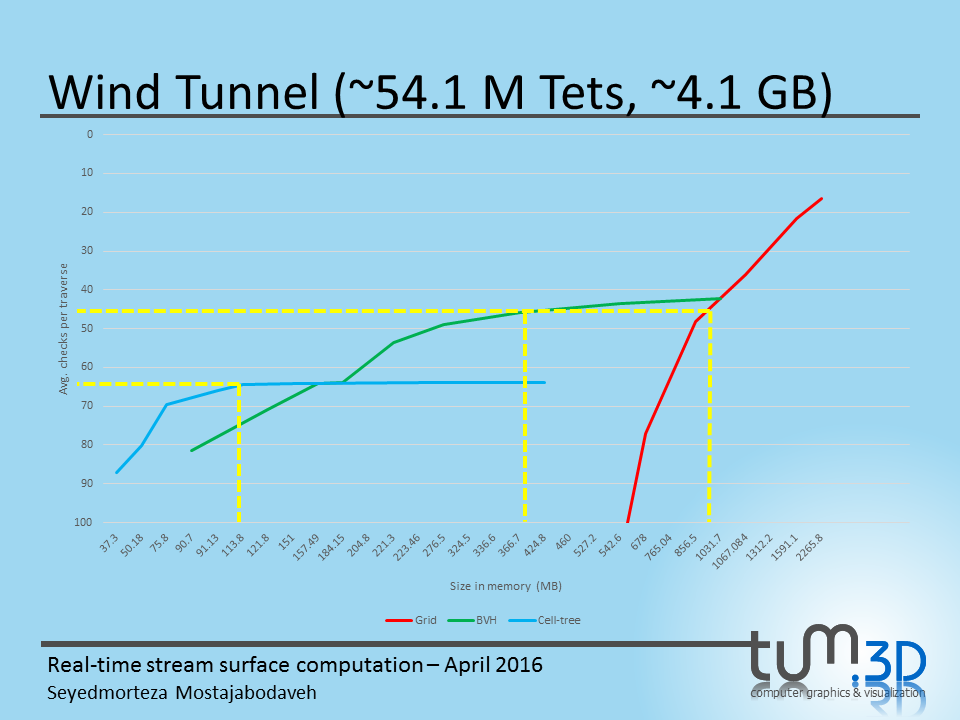
\includegraphics[height=\textheight]{figures/Slide27}
\end{frame}

\begin{frame}{Acceleration Structures Evaluation Conclusion}
	\begin{figure}[ht!]
	\centering
	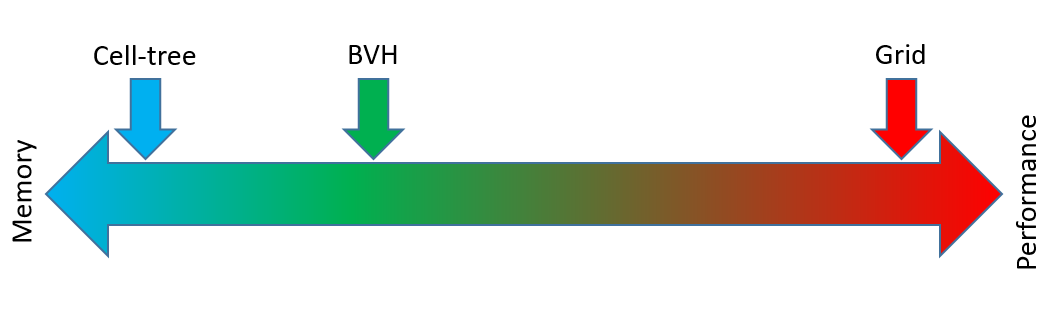
\includegraphics[height=0.2\textheight]{figures/accelstructsConclusion}
	\end{figure}
	\begin{itemize}
		\item When memory is the bottleneck \textit{Cell tree} is suitable (Cell tree size in memory is around 4-6 percent of original dataset).
		\item Highest performance is achieved using \textit{Grid} (Grid performance is higher than BVH and cell tree when its size is higher than 25 percent of original dataset).
		\item BVH seems like a balance between memory and performance (BVH size in memory in its highest performance is around 9-11 percent of original dataset).
	\end{itemize}
\end{frame}

\begin{frame}{More Information}
	\begin{itemize}
		\item More information can be found in original thesis slides and document (sent separately).
		\item Available Result Videos:
			\begin{itemize}
				\item Stream Surface in Wind Tunnel dataset: \url{https://www.youtube.com/watch?v=DmGjogQDpyE}
				\item Stream Surface in Tethrahedradecal Dataset: \url{https://www.youtube.com/watch?v=rdoRs-VpGhw}
				\item Streamlines in Telescope Dataset: \url{https://www.youtube.com/watch?v=mln05oIApY0}
			\end{itemize}
	\end{itemize}
\end{frame}

%================================================
%================================================

\section{Ray Tracing Revisited for Rendering CSG Models Consisting of Higher Order Primitives}

\begin{frame}{Outline}
	\tableofcontents[
		currentsection,currentsubsection,hideothersubsections
	]
\end{frame}

\begin{frame}{Ray Tracing Revisited for Rendering CSG Models Consisting of Higher Order Primitives}
	\begin{figure}[ht!]
		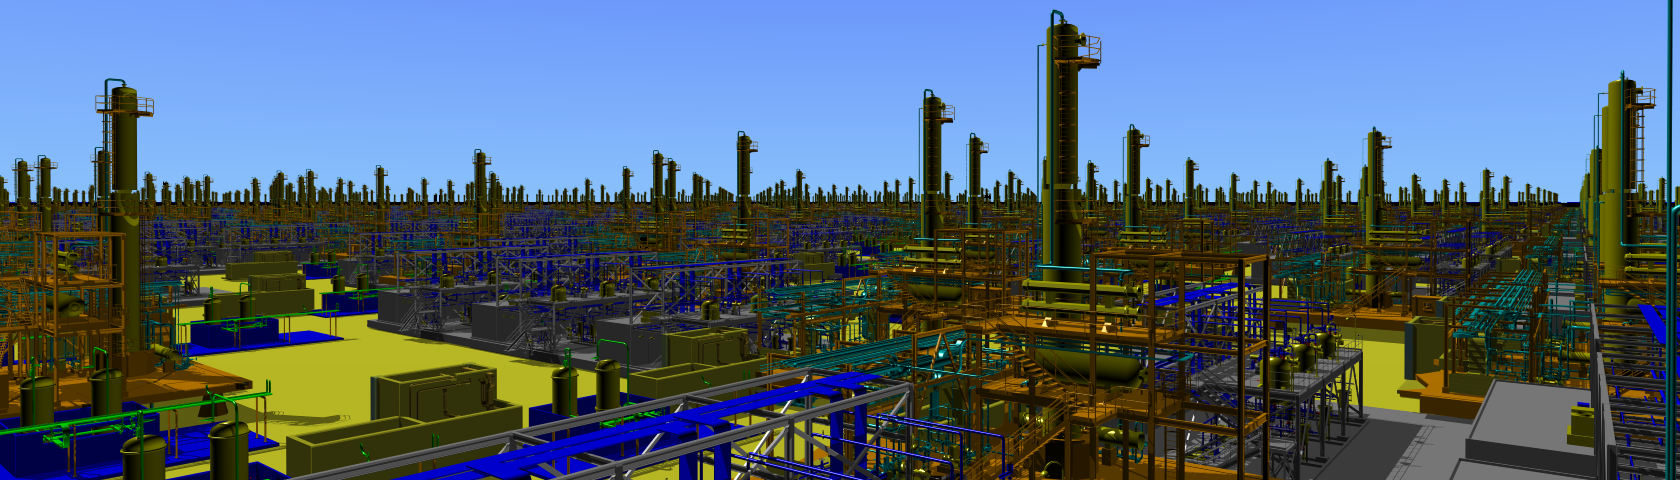
\includegraphics[width=1.0\linewidth]{figures/Plant_Teaser.png}
		\caption{
			A complex CAD scene built out of 8,000 individual plant models. In total, the scene consists of more than 100,000,000 non-planar second-order (cylinders, cones, etc.) and forth-order (tori) primitives, ray traced at more than 10~frames per second on 16 CPU
			cores, including pixel-accurate shadows.
		}
	\end{figure}
\end{frame}

\begin{frame}{Benefits}
	\begin{itemize}
		\item \textbf{On-the-fly compositing.}\\
		%
		-- Boolean set operations are performed on a per-ray basis immediately	during rendering.\\
		-- No Preprocessing.
		\item \textbf{Low storage requirement.}\\
		%
		-- small set of parameters for each primitive.\\
		-- No prior triangulation of primitives.
		-- Holding scenes in memory would be possible without triangulation.
		\item \textbf{Pixel-accurate higher order surfaces.}\\
		-- Ray-primitive intersection can be tested directly.
		-- Usually a quadratic equation which is easy to solve (tori has a quartic equation).\\
		-- No discretization artifacts are visible.\\
		-- Surfaces appear perfectly smooth.\\
	\end{itemize}
\end{frame}

\begin{frame}{Main Contributions}
	\begin{itemize}
		\item a method to apply CSG operations in real-time during ray tracing while keeping the memory overhead low.
		\item Evaluation of the proposed method in comparison to other well-known rasterization-based real-time CSG model rendering techniques(\cite{goldfeather:86:FCSGDPPGS}, and \cite{Stewart02linear-timecsg}).
	\end{itemize}
\end{frame}

\begin{frame}{Contribution: Optimized Hitpoint Calculation}
	\begin{algorithm}[H]
		\BLUECOMMENT {$ray$: current ray hitting a primitive}\\
		\vspace{0.5mm}
			\eIf{ entering primitive }
			{ $delta$ := $+1$; }
			{ $delta$ := $-1$; }

			\eIf{ positive primitive hit }
			{ $ray.posDepth$ += delta;  }
			{ $ray.negDepth$ += delta;  }

			\eIf{ ($ray.posDepth>0$) $\&\&$ ($ray.negDepth<=0$) }
			{ ReportHit(); \BLUECOMMENT{ // final hit in layer found } }
			{ ContinueRay($ray$); \BLUECOMMENT{ // still inside a negative medium } }		
		\caption{RayTraceLayer($ray$)}
		\label{alg:ray-trace-layer}
	\end{algorithm}
\end{frame}

\begin{frame}{Supported Higher Order Primitives}
	
	\begin{figure}[ht!]
		\centering
		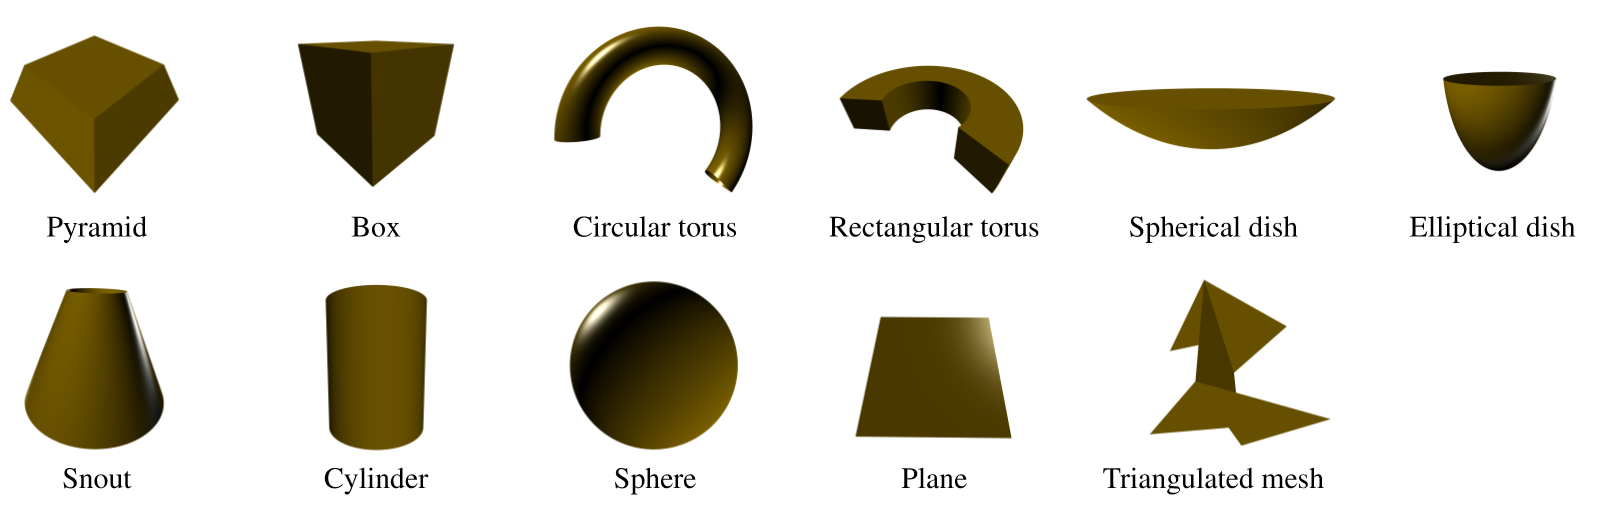
\includegraphics[width=0.9\linewidth]{figures/hops.png}
	\end{figure}
\end{frame}

\begin{frame}{More Results}	
	\begin{figure}
		\centering
		\subfigure{
			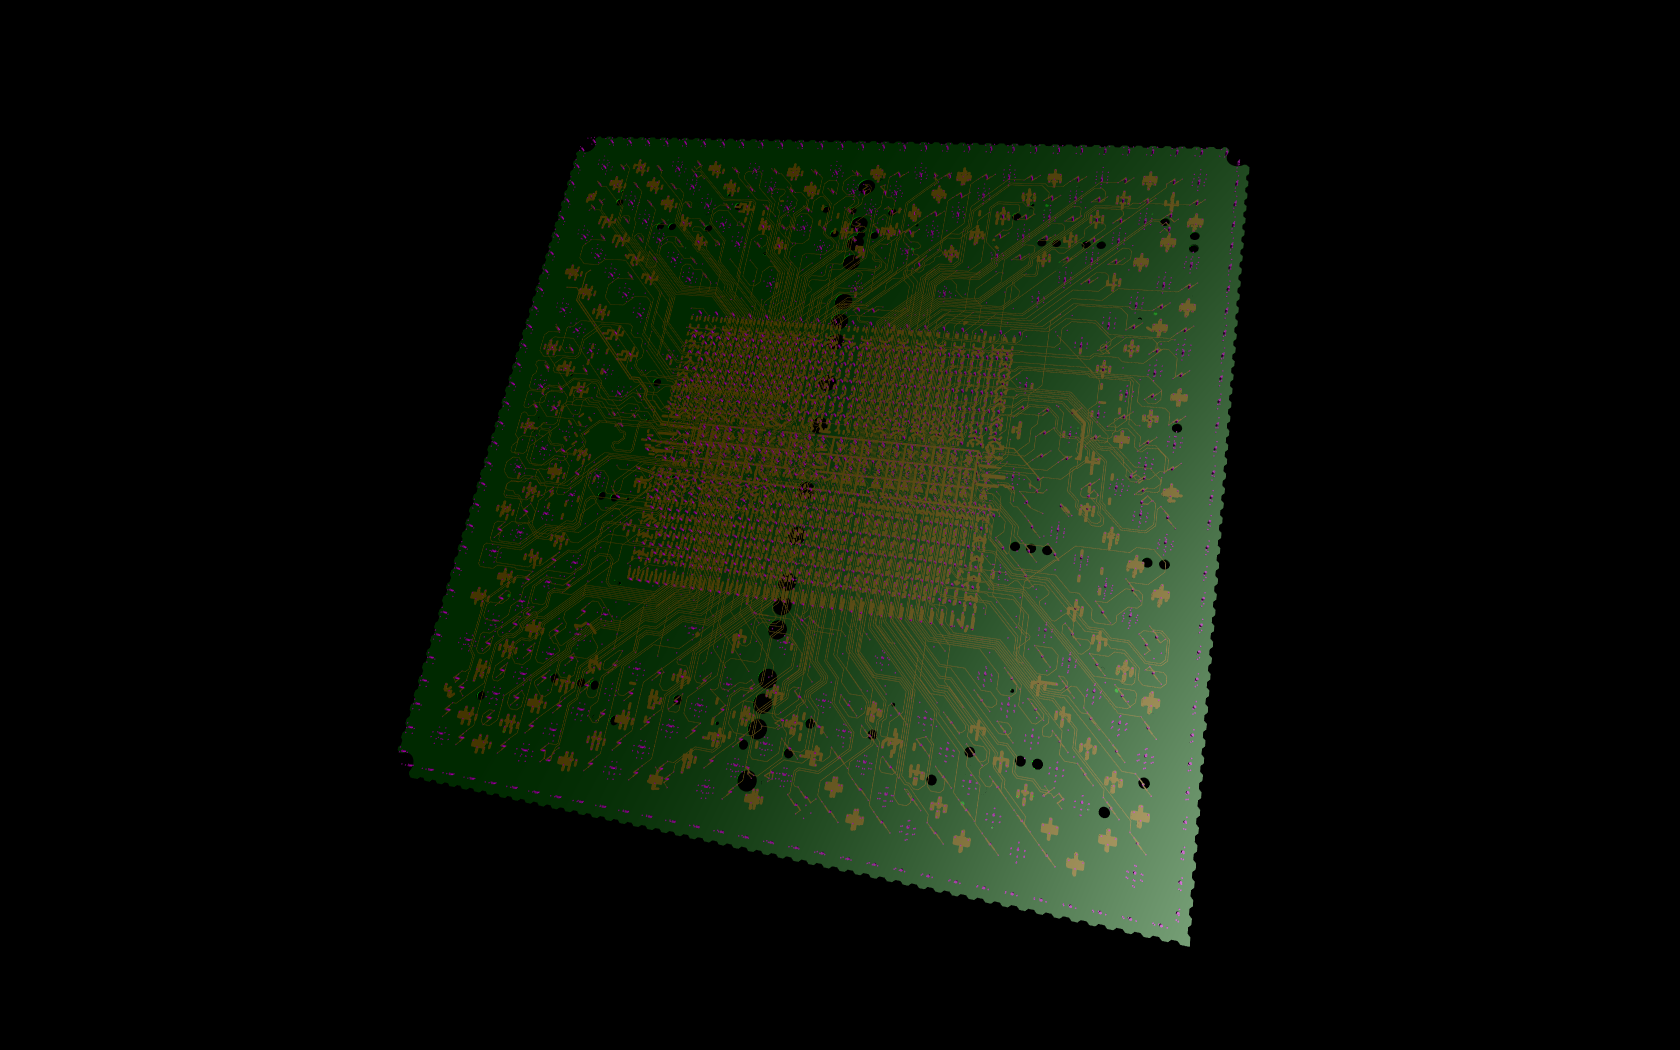
\includegraphics[width=0.45\linewidth]{figures/Plasma}
		}
		\subfigure{
			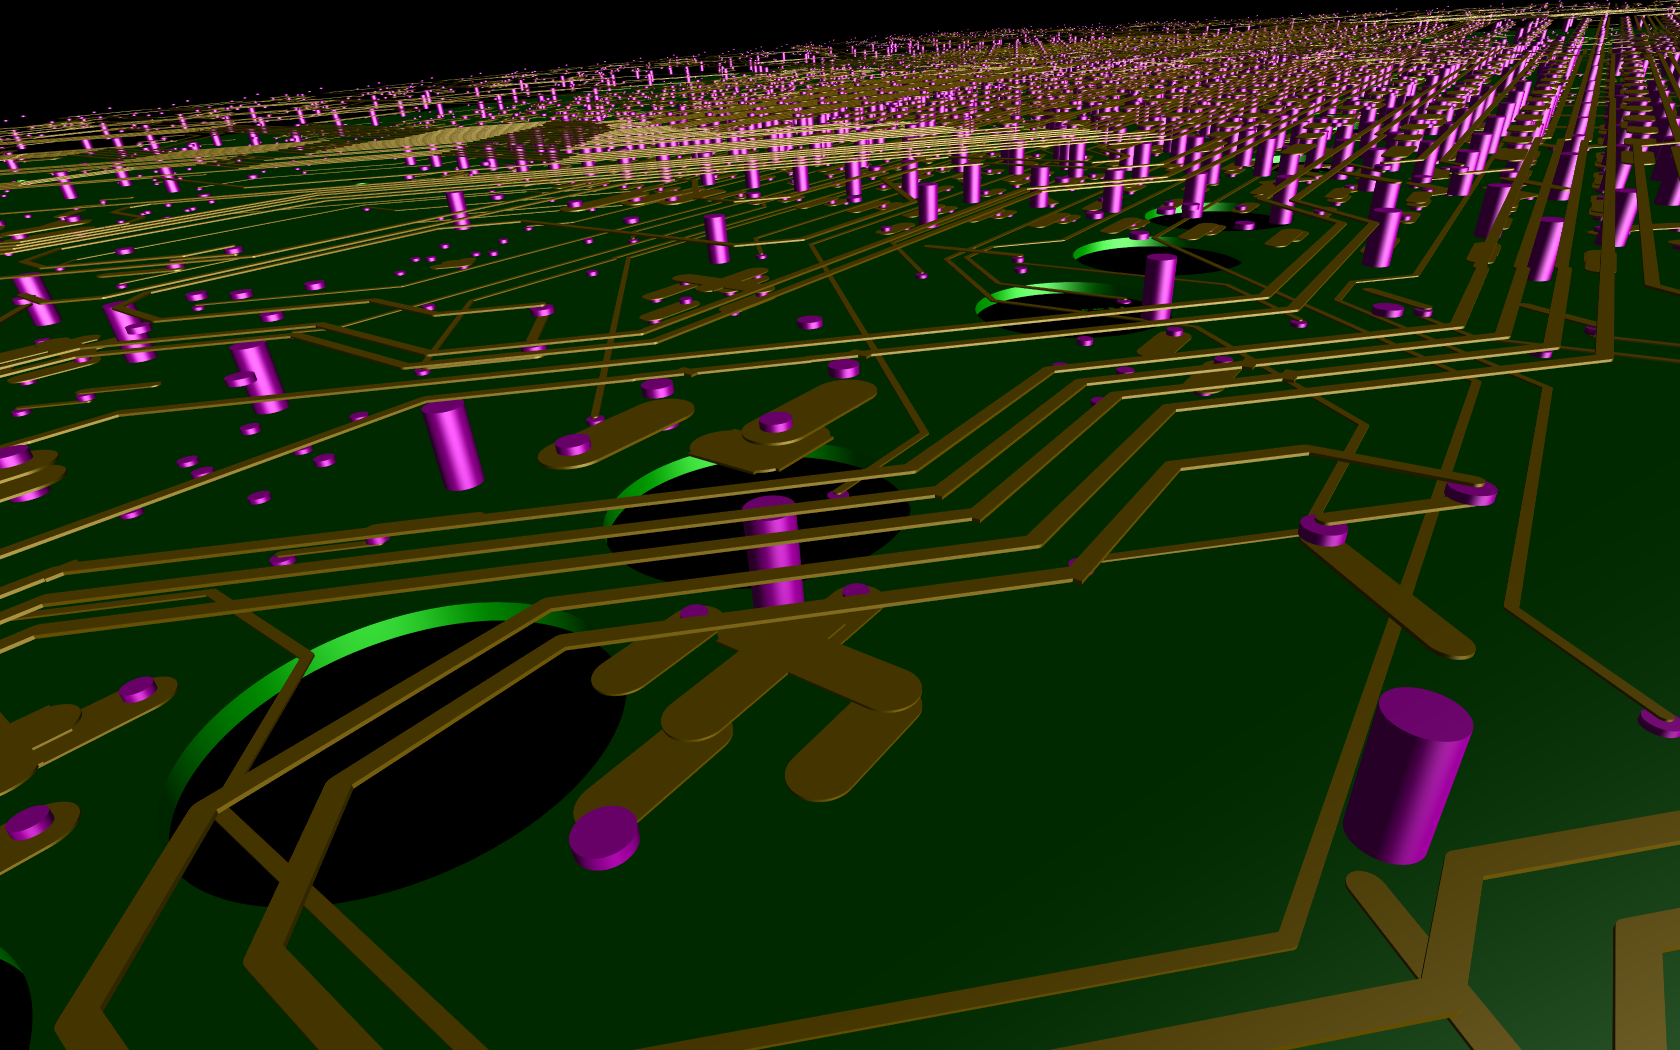
\includegraphics[width=0.45\linewidth]{figures/Plasma_Closeup}
		}\\
		\subfigure{
			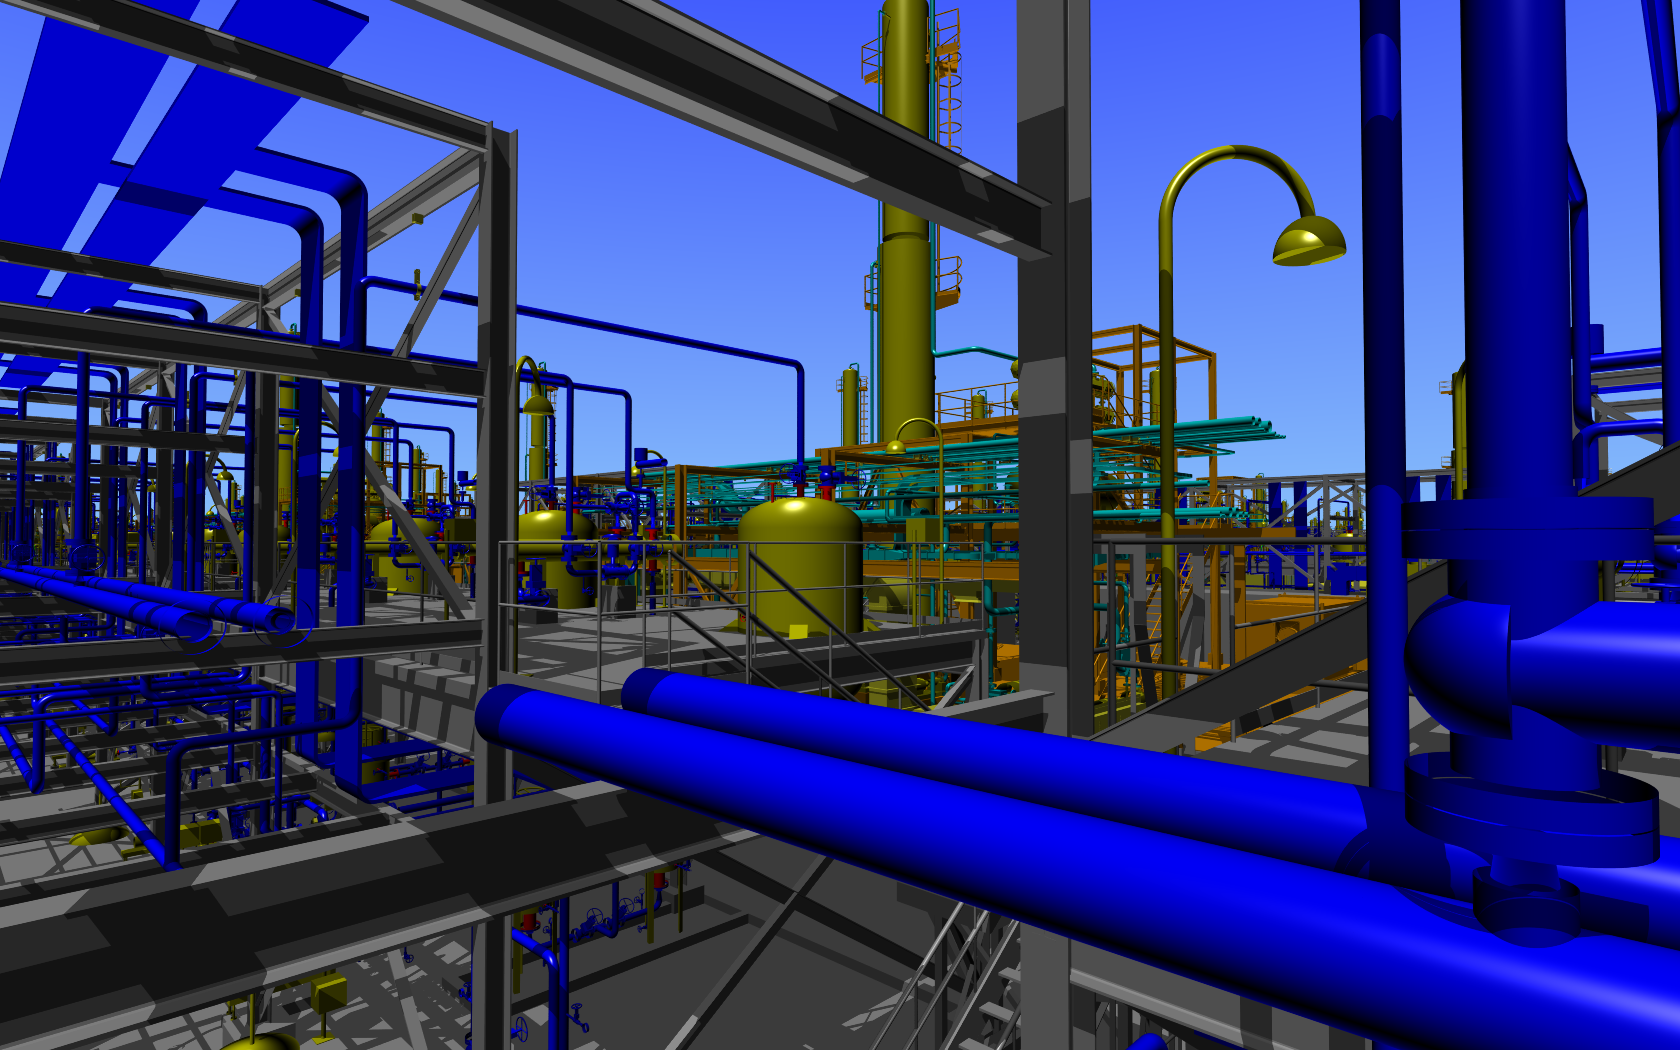
\includegraphics[width=0.45\linewidth]{figures/Plant_Closeup_1}
		}
		\subfigure{
			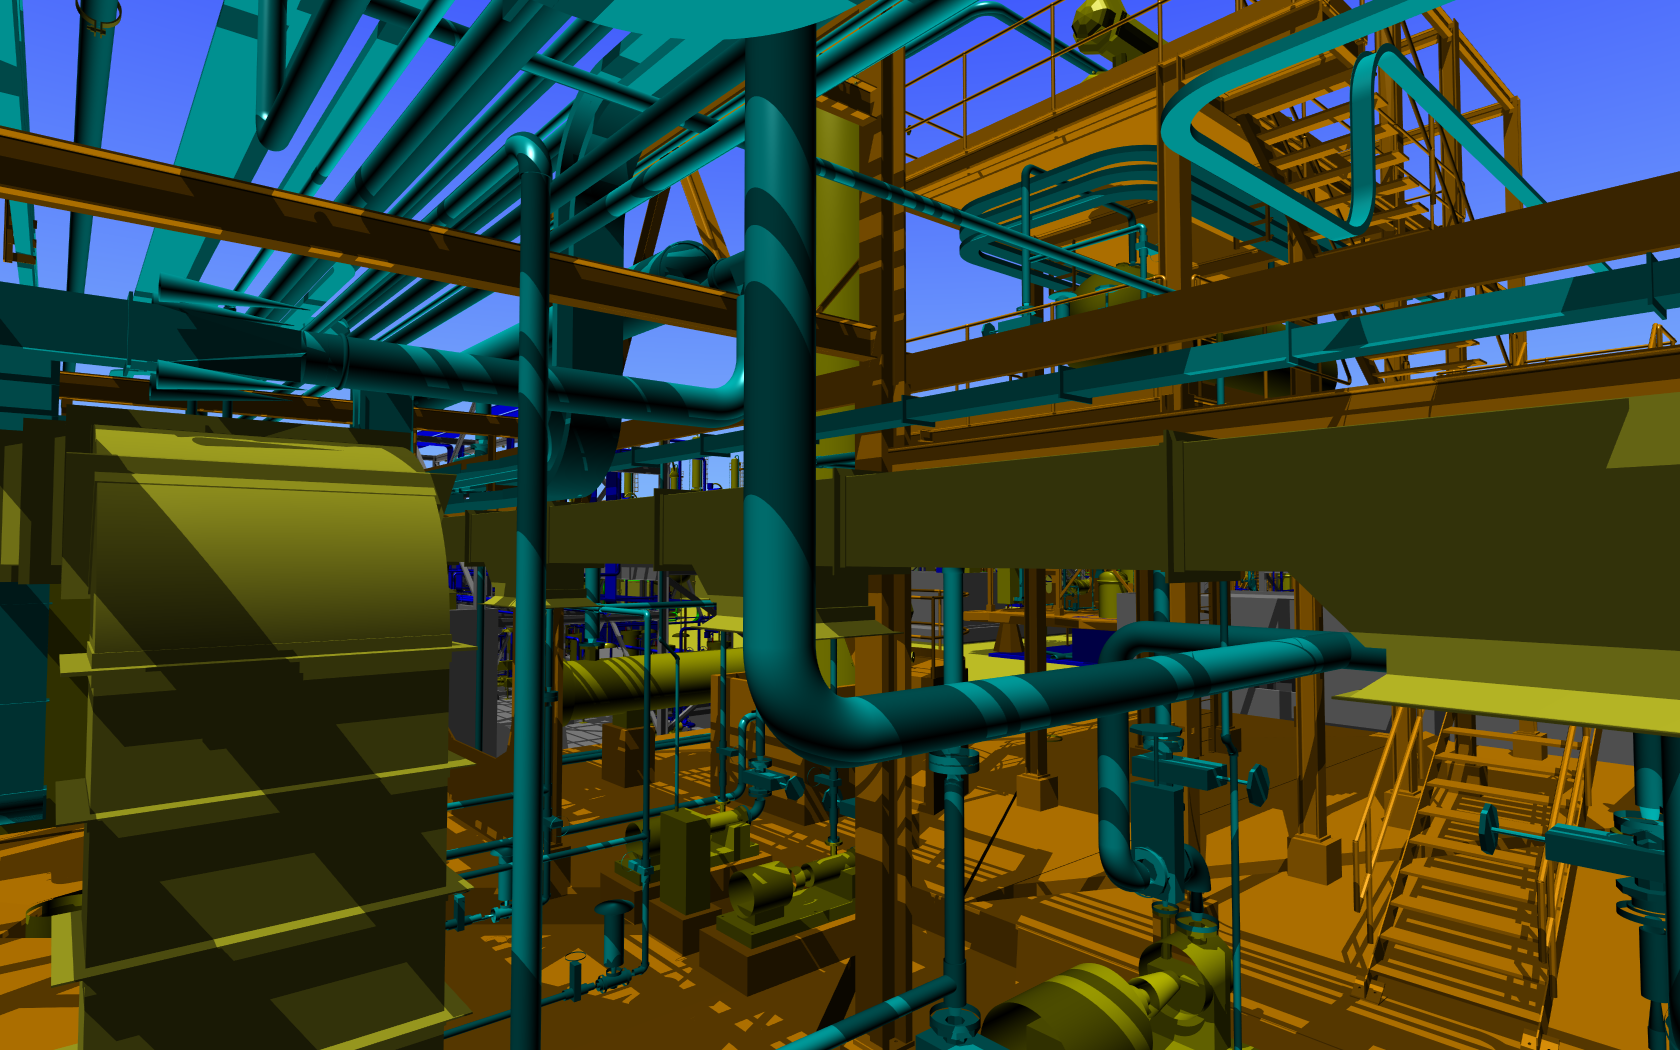
\includegraphics[width=0.45\linewidth]{figures/Plant_Closeup_2}
		}
	\end{figure}
\end{frame}

%================================================
%================================================

\section{Analysis of Voxel-Based Ray Tracing}

\begin{frame}{Outline}
	\tableofcontents[
		currentsection,currentsubsection,hideothersubsections
	]
\end{frame}

\begin{frame}{Analysis of Voxel-Based Ray Tracing}
	\begin{itemize}
		\item \textbf{Goal}: Instrumenting voxel-based path-tracer with SIMD simulator to measure ray-sorting algorithms impact on SIMD units' efficiency.
		\item  \textbf{Main Contribution}: Measure the impact of improving coherency methods (ray sorting) on instruction coherency of the rays.
	\end{itemize}
\end{frame}

\begin{frame}{Basis for Evaluations: Implementing a Voxel-Based Path-Tracer}
	\begin{figure}
		\centering
		\subfigure[Soft Shadow with Area Light]{
			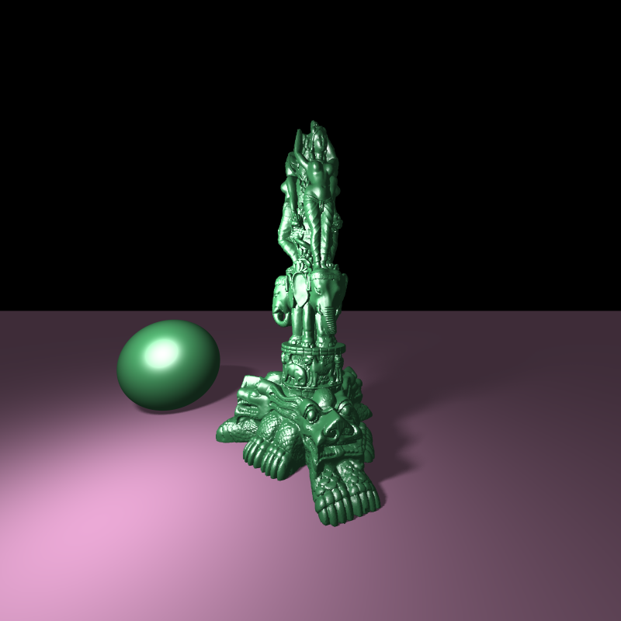
\includegraphics[width=0.3\linewidth]{figures/pathtracerResults1}
		}
		\subfigure[Global Illumination with Path Tracing]{
			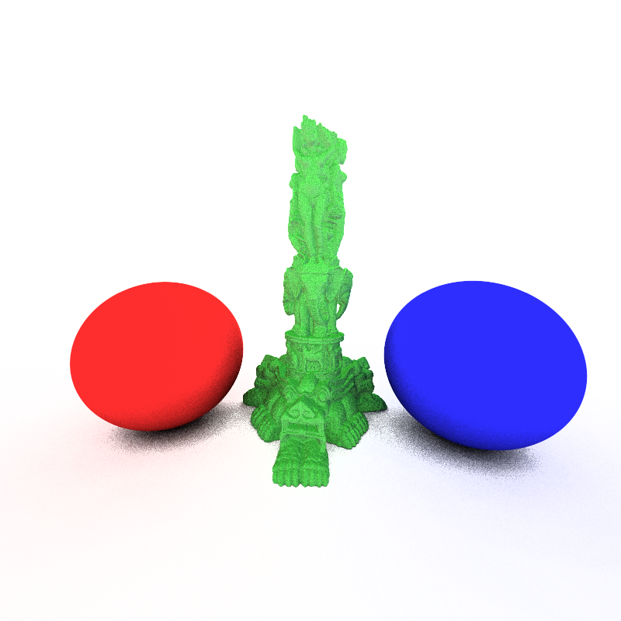
\includegraphics[width=0.3\linewidth]{figures/pathtracerResults0}
		}
		\subfigure[Cornell Box]{
			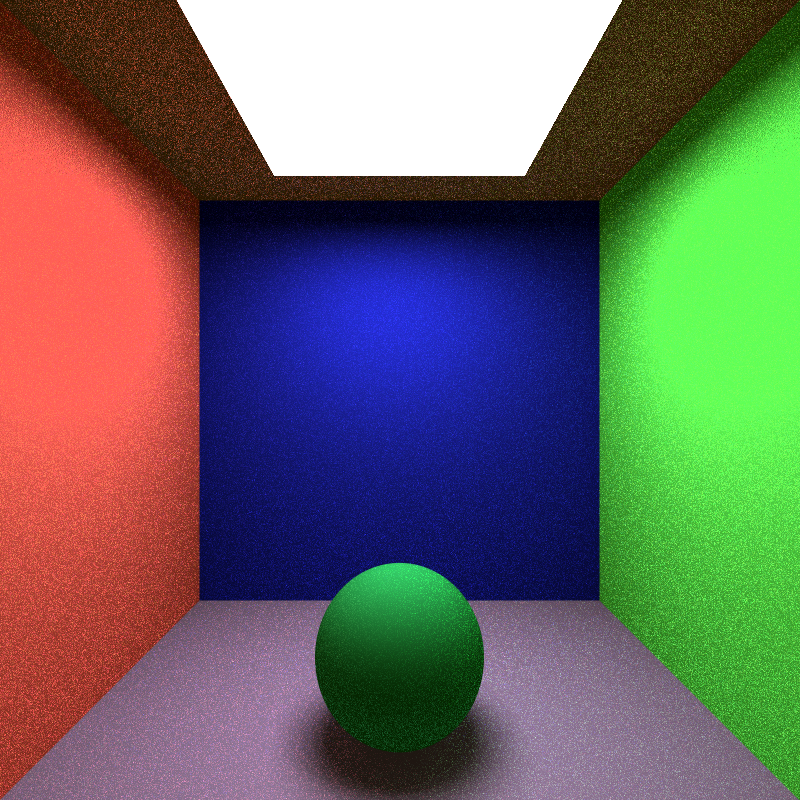
\includegraphics[width=0.3\linewidth]{figures/pathtracerResults2}
		}
	\end{figure}
\begin{center}
    All scenes are described with a hierarchy of 3d voxels.
\end{center}

\end{frame}

\begin{frame}{BVH Traversal Main Operations Classification (1/2)}
	\begin{itemize}
		\item \textbf{Push and Traverse} Ray is intersecting with both child nodes. One should be chosen and the other one should be kept in the stack.
		\item \textbf{Traverse} Ray is intersecting with one of the child nodes. The traversal path is clear.
		\item \textbf{Leaf Node Intersection} Intersection test should be done for leaf nodes.
		\item \textbf{Finished} Traversal is done.
	\end{itemize}
\end{frame}

\begin{frame}{BVH Traversal Main Operations Classification (2/2)}
	\centering
	\scalebox{0.6}{
	\begin{minipage}{\linewidth}
		\begin{algorithm}[H]
			
			%\REQUIRE Stack s is defined.
			\While{$Finished \neq true$}{
				\eIf{$CurrNode$ is $InteriorNode$}
				{
					%Check intersection with both childs of current node.\\
					\eIf{intersection with both childs}
					{
					    $NextNode \leftarrow left child$\\
						s.Push(RightChild) \textcolor{red}{\hfill Push and Traverse}\\
					}
					{
						\eIf{intersection with one child}
						{
							 $NextNode \leftarrow Intersected Child$ \textcolor{red}{\hfill Traverse}\\
						}
						{
							\eIf{not s.empty()}
							{
								$NextNode \leftarrow s.Pop()$
							}
							{
								$Finished \leftarrow true$ \textcolor{red}{\hfill Finished}\\
							}
						}
					}
				}
				{
					Intersect with voxels related to the $leafnode$ to find the intersection. \textcolor{red}{\hfill Leaf Node Intersection}\\
					\eIf{$found$ or $s.empty()$}
					{
						$Finished \leftarrow true$ \textcolor{red}{\hfill Finished}
					}
					{
						$NextNode \leftarrow s.Pop()$
					}	
				}
			}
		\end{algorithm}
	\end{minipage}%
	}
\end{frame}

\begin{frame}{Our SIMD Simulator}
	\begin{algorithm}[H]
			Reset all ray's $InstCounter$ elements to zero.\\
			$CurrStage \leftarrow 0$\\
			\While{$Finished \neq true$}
			{
				\If{All rays has done their first $CurrStage$ operations}
				{
					$CurrStage$++\\
					Continue\\
				}
				
				$CurrOp \leftarrow FindNextOperationToExecute($CurrStage)\\
				ExecuteSIMDUnitsWithNextOperation($CurrOp$)\\
				\If{Any of SIMD Units are done}
				{
					deactivate the SIMD operation unit.
				}
			}
	\end{algorithm}
\end{frame}

\begin{frame}{Example of SIMD Simulation (Instruction Coherency)}
	\begin{figure}
		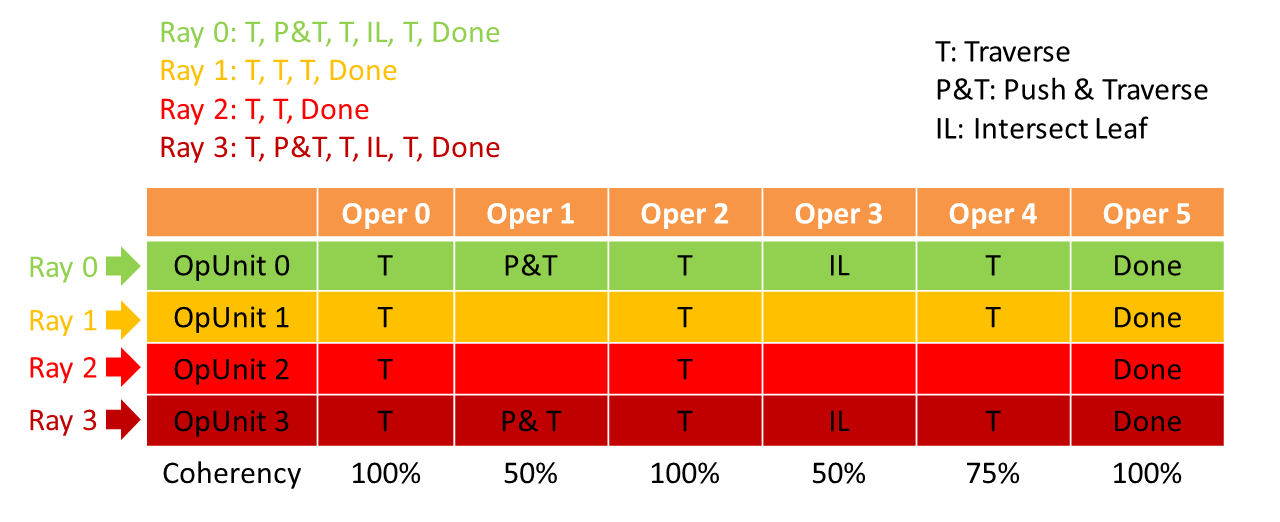
\includegraphics[width=\linewidth]{figures/SIMDExecEg}
		\caption{An example of traversing the BVH-tree for 4 different rays on SIMD of width four.}
	\end{figure}
\end{frame}

\begin{frame}{Instruction Coherency Vs. Data Coherency}
	\begin{figure}
		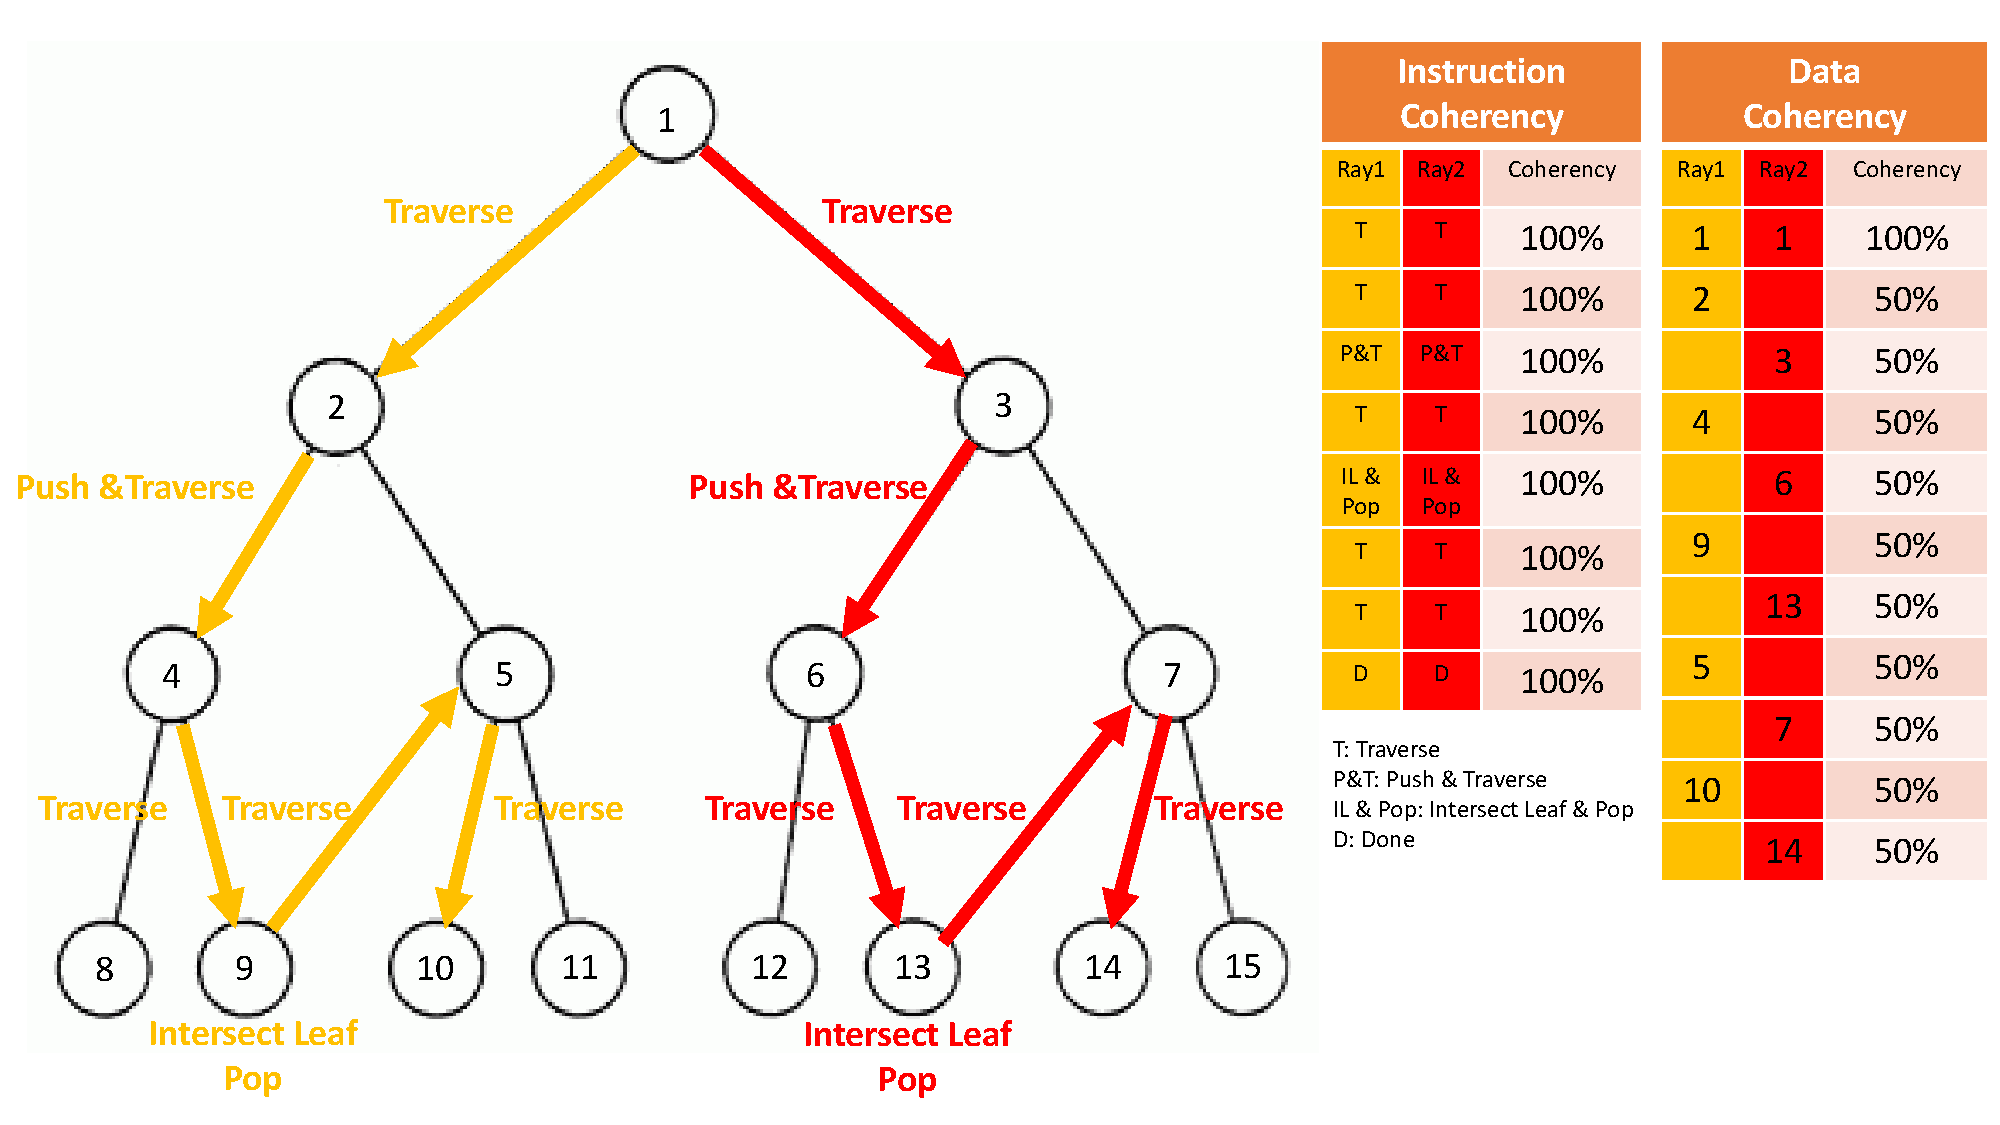
\includegraphics[width=\linewidth]{figures/InstCohEg}
		\caption{While both rays are perfectly instruction execution coherent, they are incoherent in data access.}
	\end{figure}
\end{frame}

\begin{frame}{Contribution: Coherency Measurements Results for Path-Tracing "Conference Room" (1/2)}
	\begin{table}[ht]  
		\centering % used for centering table 
		\begin{tabular}{c c c c} % centered columns (4 columns) 
			\hline %inserts double horizontal lines 
			
			Case & Primary Rays & Bounce 1 & Bounce 2 \\ [0.5ex] % inserts table 
			%heading 
			
			\hline % inserts single horizontal line 
			No Ray Sorting &  79.14\% & 49.53\% & 45.63\% \\ % inserting body of the table 
			Ray Sorting by Direction & 79.14\% & 49.70\% & 48.3\% \\ 
			Ray Sorting by Position &    79.14\% & 46.68\%  & 45.81\% \\ 
			Ray Sorting by Both & 79.14\% & 49.73\% & 48.6\% \\ [1ex]
			\hline %inserts single line 
		\end{tabular} 
	\caption{Total Ray Coherency For Different Bounces of Rays (SIMD width = 16) - Conference Room} % title of Table
		\label{table:ConfRenderCoh} % is used to refer this table in the text 
	\end{table} 
\end{frame}

\begin{frame}{Contribution: Coherency Measurements Results for Path-Tracing "Conference Room" (2/2)}
	\begin{figure}
		\centering
		\subfigure[Primarys]{
			\includegraphics[width=0.23\linewidth]{figures/GroupedHybridTraversal0}
		}
		\subfigure[Bounce 1]{
			\includegraphics[width=0.23\linewidth]{figures/GroupedHybridTraversal1}
		}
		\subfigure[Bounce 2]{
			\includegraphics[width=0.23\linewidth]{figures/GroupedHybridTraversal2}
		}
		\subfigure[Result]{
			\includegraphics[width=0.23\linewidth]{figures/conferenceRoom}
		}
		\caption{Coherency textures for the case which rays are sorted based on their direction and orientation on every bounce (SIMD width = 16). Colormap used for visualizing coherency is shown in the bottom-right corner of the figures. The range is from 0-100 percent (red-blue).}
	\end{figure}
\end{frame}

\begin{frame}{Similar Papers}
	\begin{itemize}
		\item \cite{Barringer:2014:DRS:2601097.2601222}, and \cite{pgs.20141257}
		\item They also show that while ray sorting algorithms improve ray tracing performance, they are not very effective, i.e.~hopefully new approaches can be devised to make voxel-based ray tracing even faster.
	\end{itemize}
\end{frame}

%================================================
%================================================

\section{Other Projects}

\begin{frame}{Outline}
	\tableofcontents[
		currentsection,currentsubsection,hideothersubsections
	]
\end{frame}


\begin{frame}{Practical Courses}
	\begin{itemize}
		\item Interactive Visual Data Analysis, Prof. Westermann Group.
		\item GPU Programming in Computer Vision, Prof. Cremers Group.
		\item Guided Research: Voxel-Based Path tracing, Prof. Westermann Group.
		\item Interdisciplinary Project: 3D-Visualization of electromagnetic field strength	distribution, Prof. Guenthner (F{\"o}rdertechnik Materialfluss Logistik group in TU-Munich).
	\end{itemize}
\end{frame}

\begin{frame}{Interactive Visual Data Analysis}
	\begin{itemize}
		\item Fundamental knowledge in the field of scientific visualization:
		\begin{itemize}
			\item Volume Visualization
			\item Flow Visualization
			\item GPGPU Programming
			\item Done with C++, D3D11, and HLSL.
		\end{itemize}
		\item See results as a video on: \url{https://www.youtube.com/watch?v=7pIw5PjkjmY}
	\end{itemize}
	\begin{figure}
		\centering
		\subfigure{
			\includegraphics[height=0.2\textheight]{figures/ivda1.jpg}
		}
		\subfigure{
			\includegraphics[height=0.2\textheight]{figures/ivda2.jpg}
		}
		\subfigure{
			\includegraphics[height=0.2\textheight]{figures/ivda3.jpg}
		}
	\end{figure}
\end{frame}
	
\begin{frame}{GPU Programming in Computer Vision}
	\begin{itemize}
		\item Implementing \textit{Optical Flow} on GPU\\
		\begin{figure}
			\centering
			\subfigure{
				\includegraphics[height=0.25\textheight]{figures/optical_flow_a}
			}
			\subfigure{
				\includegraphics[height=0.25\textheight]{figures/optical_flow_b}
			}
			\subfigure{
				\includegraphics[height=0.25\textheight]{figures/optical_flow_c}
			}
		\end{figure}
		\item Implementing \textit{Super Resolution} on GPU \\
		\begin{figure}
			\centering
			\subfigure{
				\includegraphics[height=0.35\textheight]{figures/super_resol_a}
			}
			\subfigure{
				\includegraphics[height=0.35\textheight]{figures/super_resol_b}
			}
		\end{figure}
	\end{itemize}
\end{frame}

%\begin{frame}{Guided Research: Analysis of Voxel-Based Ray Tracing}
%	Described in previous slides...	
%\end{frame}

\begin{frame}{Interdisciplinary Project: Implementing a Framework for 3D Visualization of Electromagnetic Field Strength Distribution}
	\begin{itemize}
		\item Build a model of examined installation in 3d virtual world.
			\begin{itemize}
				\item fast and intractable (Using tracking system)
			\end{itemize}
		\item Visualizing 3d bars in virtual world to specify amount of data collected in each area.
		\item Visualizing collected data using different techniques.
			\begin{itemize}
				\item Goal: Detecting weak/strong magnetic fields in different parts of environment.
				\item Visualizing data using torus and sphere glyphs.
				\item Visualizing data using direct volume rendering.
			\end{itemize}
	\end{itemize}
\end{frame}

\begin{frame}{Interdisciplinary Project: Implementing a Framework for 3D Visualization of Electromagnetic Field Strength Distribution}
	\begin{figure}
		\centering
		\subfigure[Torus Glyph]{
			\includegraphics[width=0.30\linewidth]{figures/idp2}
		}
		\subfigure[Sphere Glyph]{
			\includegraphics[width=0.30\linewidth]{figures/idp1}
		}
		\subfigure[Direct Volume Rendering]{
			\includegraphics[width=0.30\linewidth]{figures/IDP_dvr}
		}
	\caption{Different visualization techniques used in this project (screenshots are not captured in for the same data).}
	\end{figure}
\end{frame}

\begin{frame}{Related Courses}
	\begin{itemize}
		\item Computer Graphics related: Computer Graphics, Image Synthesis, Scientific Visualization, Augmented Reality, Computer Animation and Simulation.
		\item Parallel Programming related: Parallel Programming, Advanced Computer Architecture.
	\end{itemize}
\end{frame}

%================================================
%================================================

\section{Discussion}

\begin{frame}{Outline}
	\tableofcontents[
		currentsection,currentsubsection,hideothersubsections
	]
\end{frame}

\begin{frame}{Discussion}
	\begin{itemize}
		\item Prof. Slusallek: What do you want to be known for in next 5 years?
		\item Me: I like \textbf{real-time rendering}. I would like to be known for improving rendering for \textbf{virtual reality} applications.
		\item Prof. Slusallek: Are you mostly interested in implementation or theory?
		\item Me: I like theories and try to study and understand them but I am mostly interested in \textbf{implementation}-wise works.
	\end{itemize}
\end{frame}

%================================================
%================================================

\section{Current Status}

\begin{frame}{Outline}
	\tableofcontents[
	currentsection,currentsubsection,hideothersubsections
	]
\end{frame}

\begin{frame}{Current Status}
	\begin{itemize}
		\item Working at Fraunhofer IGD, Darmstadt as a Researcher.
		\item Involved in two projects:
			\begin{itemize}
				\item \textbf{VELaSSCo EC Funded Project} (\url{http://www.velassco.eu/}).\\
				
				-- Our simulation models are stored in a Hadoop database (HBase) which is running on a HPC.\\
				-- Idea: Doing post processing (mesh simplification, and streamline computation) on the HPC and send the result as triangle mesh for the client.\\
				-- My task is to implement Fraunhofer IGD's visualization client, some of data access queries on HPC side, and streamline computation post processing technique on the HPC side using map-reduce.
				\item an industrial project in collaboration with CST AG.\\
				-- Worked on dynamic tessellating arc primitives in real-time on CPU and upload the triangles to the GPU.
				\item \textbf{Both projects will be over soon (end of February 2017 is the final VELaSSCo review meeting) and that's a great time to leave Fraunhofer IGD :)}
			\end{itemize}		
	\end{itemize}
\end{frame}

\begin{frame}[allowframebreaks]
	\frametitle{References}
%	\bibliographystyle{amsalpha}
	\bibliographystyle{apalike}
	\bibliography{bibliography}
\end{frame}


\end{document}